\documentclass[12pt,a4paper,twoside]{report}

\usepackage[lmargin=2.54cm,tmargin=2.54cm,rmargin=2.54cm,bmargin=2.52cm]{geometry}
\usepackage[utf8]{inputenc}
\usepackage[T1]{fontenc}
%\usepackage{cite}

\usepackage{mathptmx}
\usepackage{fancyhdr}
\usepackage{graphicx}
\usepackage{subcaption}
\usepackage{pdfpages} 
\usepackage{amsmath}
\usepackage{lipsum}
\usepackage{mwe}

%\usepackage{showframe}
%\usepackage[citestyle=alphabetic,bibstyle=authortitle]{biblatex} 
%\addbibresource{ProjectResearchPapers.bib}
\usepackage{hyperref}

\hypersetup{
	colorlinks,
	citecolor=black,
	filecolor=black,
	linkcolor=black,
	urlcolor=black
}

\pagestyle{fancy}
\fancyhf{}
\fancyhead[LE,RO]{The University of Sheffield}
\fancyhead[RE,LO]{Akinola Alexander Dada}
\fancyfoot[CE,CO]{\thepage}
\fancyfoot[LE,RO]{Master's Dissertation}
\fancyfoot[RE,LO]{ACSE}

\linespread{1.5}

\title{ Modelling, Simulation, and Implementation of Linear Control for Asymmetric Multirotor Unmanned Aerial Vehicles}
\author{Akinola Alexander Dada \\ Reg No.160140802}
\date{$\today$}

\pagenumbering{roman}
	
\begin{document}

	\begin{abstract}
		Unmanned Aerial Vehicles (UAVs) are aerial systems not directly controlled by onboard personnel. There are many types of UAV platforms, chiefly defined by the characteristics of their mechanical constructions. One such class of UAVs are multirotors which possess multiple rotor wing actuators. These types of UAVs have a wide range of applications due to their ability to perform vertical/Short take-off and landing (VSTOL), stationary and low speed flight, coupled with their relatively simple mechanical designs when compared to single rotor constructions. The major challenge in dealing with these types of UAVs is their inherent instability in flight, save for the intervention of complex control systems. Therefore, in order to understand control systems capable of producing guaranteed performance, this project first seeks to investigate the physical characteristics and responses of UAVs through mathematical modelling, before proceeding to, design, develop, implement and compare the performance of 2 advanced linear control schemes on an embedded microprocessor, where this level of insight is requisite. These control schemes are, Linear Quadratic Gaussian (LQG) and Linear Quadratic Model Predictive Control (LQ-MPC). 
	\end{abstract}
	\newpage
	
	\section*{Executive Summary}
	
		The first chapter provides a project introduction containing background information pertinent to the investigation, briefly discussing the nature and potential uses of UAVs. This section includes the systems engineering approaches taken, such as breaking down the project aims and objectives and setting them up as a set of tasks with milestones. This section provides information on project planning and management which includes the use of Gantt charts. This section will also detail all considerations and changes made to the project including those due to the SARSCOVID-2 pandemic.
		\\ \\
		The second chapter reviews and provides an analysis of the relevant supporting literature collected, which is referenced throughout the writing. The supporting research materials take the form of scientific journals articles, independent research publications, exerts from university lectures, and published books.
		\\ \\
		The third chapter briefly discusses the mechanical design and construction of the specific asymmetric hexarotor UAV being used as the case study. This Section goes through and details the processes and results of analysing the UAV and deriving a mathematical representation of the physical characteristic through a combination of first principles dynamic modelling and hardware-in-the-loop (HIL) testing. This section explores and expatiates on different modelling techniques while discussing the various assumptions made during the modelling process, a well as the reasoning behind the adopting of the techniques selected. This section then converts the derived model into various forms useful for control design, analysis and simulation.
		\\ \\
		The forth chapter presents an analyses of the system characteristics along with a dynamic simulation using industry standard applications. This section details the process behind the design and development of an LQG feedback controller, then discusses and analyses the simulation results. This section then discusses the limitations of LQG controllers prompting and justifying the design and development of an LQ-MPC feedback controller. This section presents and analysing the simulation results of the LQ-MPC feedback controller. This section then compares the performance of the LQG and LQ-MPC feedback controllers using appropriate metrics.
		\\ \\
		The fifth chapter discusses the characteristics of the embedded Linux single board computers (SBCs), using the BeagleBone Blue platform as a case study. This section discusses and details the processes and considerations behind implementing a UAV flight control systems on the platform. The section then presents a Unified Modelling Language (UML) Class diagram detailing an implementation proposal for an embedded LQG Controller.
		\\ \\
		The sixth and final chapter concludes and summarises the investigation results then presents possibilities for future work and development.
		
	\newpage
	
	\tableofcontents
	
	\newpage
	
	\listoffigures
	
	\newpage
	
	\listoftables
	
	\newpage
	
	\pagenumbering{arabic}
	
	\chapter{Introduction}
		
		\begin{enumerate}
			\item
				Background.
			\item 
				Aims and Objectives. 
			\item 
				Project Management.
		\end{enumerate}

		\section{Background}
		
			UAVs are aerial systems which are not directly controlled by a human onboard the vehicle. There are many types of UAV platforms which are chiefly defined by the characteristics of their mechanical constructions \cite{3},\cite{4}. These defining criteria break down to include:
			
			\begin{itemize}
				\item
					The position, number and type of their actuators.
				\item 
					Their mode/modes of flight. 
				\item 
					Their use cases specific features.
			\end{itemize}
			\space
			One such type of UAVs are multirotors, defined as such due to their multiple rotor wing actuators. UAVs of this description were developed in response to the mechanical complexity of single or dual rotor winged aircraft such as the various helicopter and auto-gyros variants. Despite both classes of UAVs possessing the ability to perform operations requiring VTOL, stationary and low speed flight, the greater simplicity of multirotor craft could potentially lead to reduced development, construction and maintenance costs as well as greater reliability in use \cite{12}.
			\\
			These features enable them to be utilised in many wide ranging applications, where great dexterity in motion is required, and as such would not be possible using fixed winged platforms, such as operations required during; directed precision administration of substances to plants in precision agriculture, frequent and or detailed inspection of standing structures, precision wide area surveillance, amongst many others \cite{6}.
			\\
			However, the major challenge in dealing with multirotor UAVs is their inherent instability in real world flight situations, where disturbances are present, making it impossible to operate these craft with direct open loop control of their actuators, as is possible and frequently done with fixed winged craft. Therefore, the need for the development of control systems is apparent. 
			\\
			In order for the developed control systems to behave in a guaranteed predictable manner and be able to meet defined performance specifications, it becomes necessary to understand the behaviour of the system to be controlled and thus derive a behavioural representation to be used in guiding and informing the design process, which is done through mathematical systems modelling. This level of insight is also required in the development of advanced control schemes.
		
		\section{Aims and Objectives}
			
			The framework of this project was set around the design and development of control software for VSTOL model aircraft. From this broad theme, the aims of modelling an asymmetric multirotor platform, developing multiple control schemes and then implementing these schemes on via an embedded SBC were derived.
			\\
			These aims break down into multiple objectives and milestones which must each be achieved to fulfil the full scope of the aims outlined. These objectives can be broadly classified into 2 categories: 
	
				\subsection{Basic Objectives}
				
					\begin{enumerate}
						\item
							Develop a mathematical model representing the dynamics of the multirotor aircraft.
						\item
							Develop a dynamic simulation of the crafts behaviour.
						\item
							Develop LQG feedback control.
						\item
							Investigate feedback control laws in simulation with the mathematical model to achieve behavioural targets.
						\item
							Develop flight control software to interface with sensors and implement control laws.
						\item
							Implement the flight control software on an embedded microprocessor unit(**).
						\item
							Discuss the results of performance comparisons between the simulation and hardware implementations(**).
					\end{enumerate}
				
				\subsection{Advanced Objectives}
				
					\begin{enumerate}
						\item
							Investigate the application of LQ-MPC schemes in simulation.
						\item	
							Incorporate and implement LQ-MPC schemes unto the flight control software(**).
						\item	
							Discuss the differences between the LQG and LQ-MPC implementations.
					\end{enumerate}
				
		\section{Project Management}
			
			\begin{figure}[h!]
				\centering
				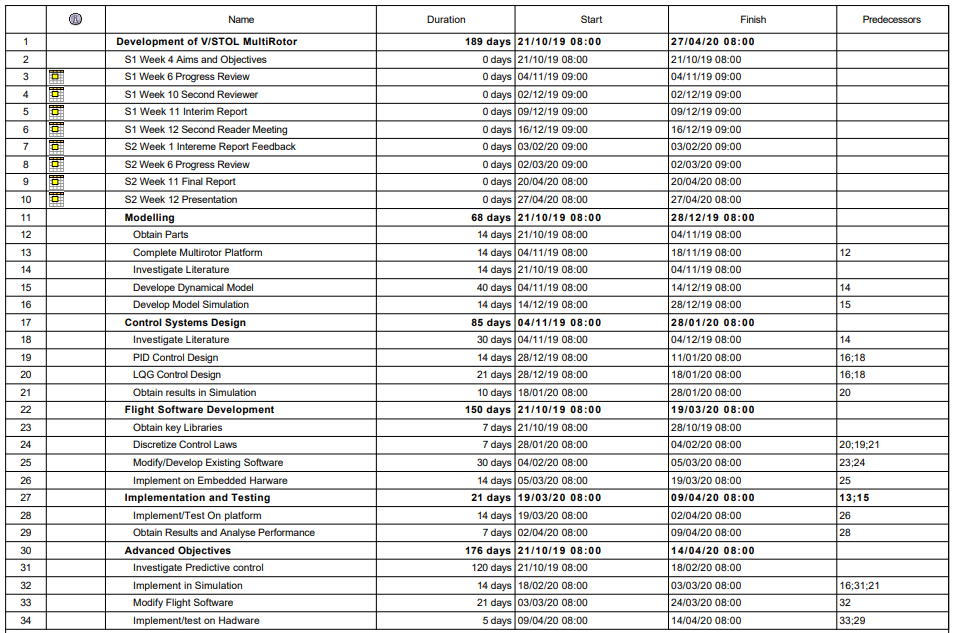
\includegraphics[width=1.1\linewidth]{ProjectInitialTimetable.png}
				\caption{Initial Timetable}
				\label{fig:initialtimetable}
			\end{figure}
		
			\begin{figure}[h!]
				\centering
				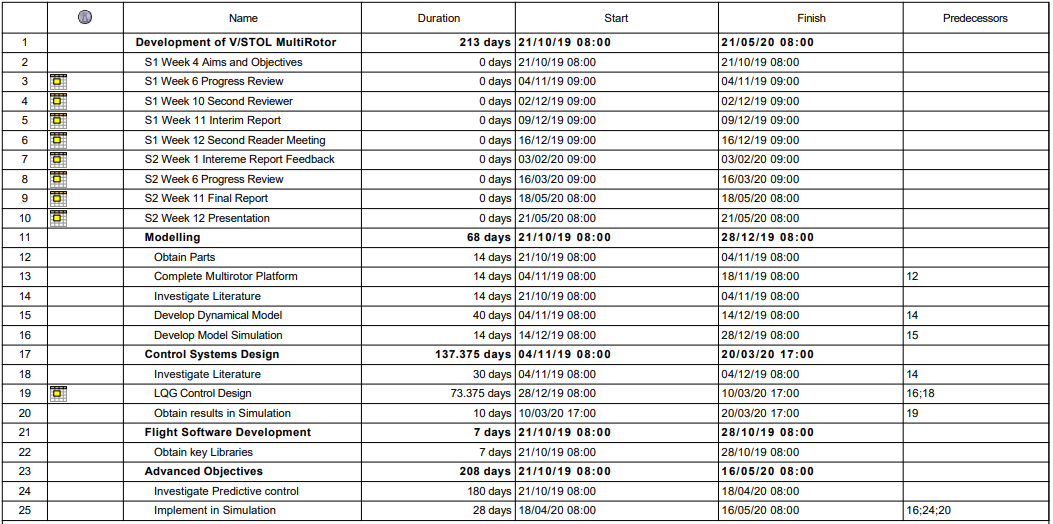
\includegraphics[width=1.1\linewidth]{ProjectFinalTimetable.png}
				\caption{Final Timetable}
				\label{fig:finaltimetable}
			\end{figure}
		
			In order to properly execute on the project Aims and Objectives, project activities were coordinated and managed by further breaking down and grouping tasks then laying them out in tabulations, Figures 1.1 and 1.2, which were used to generate the project Gantt charts showing required progress against time.
			\\ \\
			Due to the effects and responses to the global SARSCOVID-2 pandemic, The University of Sheffield was forced into closure/Cancellation of all on-site and in-person teaching, meetings and instruction from March of 2020. This coupled with the government mandated nationwide quarantine and lock down in the United Kingdom made access to the necessary facilities for the testing and evaluation of any developed UAV software impossible. As such, activities and work towards meeting the objectives succeeded by Double-Asterix in the aims and objectives subsection are not being undertaken. Project planning has been adjusted accordingly. This has also led to changes in term dates which resulted in adjustments being made to task timelines.
			\\ \\
			Regarding other aspects of the project, all material purchases were made on time, acquiring key hardware such as the main flight computer, the flight radio control system, which would have served as the main communication unit sending control commands to the multirotor, electronic speed controllers, and load cells which will be used to develop the test stand platform to identify the actuator dynamics. All Ad hoc minor changes to task completion periods are reflected in timeline changes from the initial proposal table, Figure 1.1, to the final proposal table, Figure 1.2. 
			\\
			The only major change to the project scope, not enforce by SARSCOVID-2, from its initial proposal, was the dropping of a PID control design section and all such tasks, which occurred before, and is reflected in, the S2 week project proposal review. This change was made to refocus the project objectives solely on model-based control design outcomes.
			\\ \\
			All changes to task completion dates for further objectives are displayed in the final proposal table, Figure 1.2, which was used to produce the final project Gantt chart available in Appendix A.
			
	\newpage
	
	\chapter{Review Of Literature}	
	
		\section{Introduction}
		
			In preparing to execute the project tasks, various supporting and reference materials were acquired. The various reference literature take the form of articles published in scientific journals, research publications, exerts from university lectures, and published books, all of which together broadly cover and present 3 major themes that are relevant to the project’s investigation:
		
			\begin{enumerate}
				\item 
					Mathematical Modelling and Systems Identification. 
				\item 
					Control Systems Design.
				\item 
					Simulation and Implementation.
			\end{enumerate}
		
		\section{Mathematical Modelling and System Identification}
			
			\subsection{UAV}
				
				The exact details involved with the design, development and construction of UAVs is beyond the scope of the investigation but material, mechanical and electronic consideration when designing such craft are explored in \cite{12}.
				
			\subsection{Dynamics}
			
				In modelling systems, it is first necessary to state all assumptions made about its characteristics. These assumptions simplify the process of systems model abstraction. Following that, multirotors can be defined as rigid-bodies free to move in three-dimensional (3-D) space, therefore, moving with 6 degrees of freedom (6-DOF). With this modelling assumption, UAV motion is subject to the laws of rigid body Kinematics and Kinetics. All the acquired material takes this stance. 
				\\
				Vehicle motion is defined in terms of 2 coordinate frames moving relative to one another where the physical quantities that change with time, called states, change with respect to one frame or the other. They are the Earth-Frame, fixed to the earth and the Body-Frame, attached to the vehicle body. Each frame consists of 3 orthogonal axes, whose nomenclature varies from source to source, about and along which rotational and translational motion can occur respectively \cite{1},\cite{2},\cite{4},\cite{15}. 
				\\
				The sources obtained explore 2 ways for representing this rotational motion of the reference frames:
				
				\begin{itemize}
					\item 
						Sources \cite{1},\cite{2},\cite{3},\cite{4},\cite{5},\cite{6},\cite{7},\cite{9} present their models using Euler angles which describe arbitrary orientation in the 3-dimensional Euclidean space using three parameters which represent a sequence of three elemental rotations about each axes of the coordinate system. Any orientation in 3D space can be achieved by composing these 3 elemental rotations.
					\item
						Sources \cite{1},\cite{8},\cite{16} present representations through Quaternions which solve issues present with computing Euler angles such as computational expense and numerical singularities which occur when certain orientations are reached, as Quaternions do not require the calculation of sin and cos when certain angles go to 0 or 90 degrees and their multiples. Quaternions represent any arbitrary orientation by constructing rotations as that of a single angle about an imaginary axis. 
				\end{itemize}
				\space
				The rigid body assumptions also allow for the utilisation of several Mechanical Modelling techniques and conventions which are used to derive the non-linear dynamics of the body frame mechanical systems considering both kinematics and Kinetics:
				
				\begin{itemize}
					\item
						The Newton-Euler convention which derives representations of systems dynamics through the application of first principles using newtons 2nd law of motion showing the effects of forces applied to the rigid body by its actuators and environment. Utilised in \cite{2},\cite{3},\cite{5},\cite{6},\cite{7},\cite{8},\cite{9}.
					\item 
						The Euler-Lagrange convention which derives representations of systems dynamics through the study of energy differentials between kinetic and gravitational potential generated by motion. Utilised in \cite{4}. 
					\item 
						The Newton-Hamiltonian.
					\item 
						Pure Hardware-in-the-Loop system identification, which decouples each axes of motion and determines approximate model frameworks for each then populates said framework with experimentally obtained parameters. Such was the process taken by \cite{28}
				\end{itemize}
				\space
				This investigation utilises the Euler-angle representation and the Newton-Euler convention due to its intuitive familiarity and relative simplicity.
				\\
				Due to the UAV's layout, it is asymmetric, this creates a system where its mass is not geometrically evenly distributed about the centre of mass leading to where inertia is not represented by a typical diagonal inertial tensor but instead one with non-trivial off diagonal elements and thus creating transposed reference frames. However, for the purpose of this investigation, it is assumed that the system is symmetrical as the off-diagonal terms in the inertia matrix are far lower in magnitude than the diagonal terms, thus can be reasonably neglected. Otherwise, the entire coordinates system would be adjusted and transformed to produce a true diagonal matrix as presented in \cite{10}. 
				\\ \\
				In order to design the controllers, the non-linear model obtained via the Newton-Euler convention needs to be linearised. This is accomplished through the application of Jacobi’s linearisation method as presented in \cite{11}. This process produces a full linear state space representation of systems dynamics around stable operating points. This model is then discretized for analysis and implementation in digital embedded systems.
				
			\subsection{Actuator Dynamics}	
			
				The UAV is actuated by 6 1000Kv brushless direct current (BLDC) motors \cite{14}, attached to 6 10x45inch propellers and is powered by a 4-cell lithium-polymer battery with an operational voltage range of 16.8 volts to 12.8 volts. To fully develop a system model, the characteristics of these parts must be modelled. This can either be done via first principles calculations as presented in \cite{2},\cite{8},\cite{17} or via experimental systems identification as presented in \cite{9},\cite{12},\cite{14},\cite{15},\cite{16}. 
				\\
				The systems identification approach involves the derivation of a lumped parameter linear input-output model, encompassing the electronic speed control unit, motor and propeller dynamics, between input Pulse width modulated (PWM) signal pulse width and the output angular velocity, torque and thrust forces. This has the advantage of reducing complex dynamics enabling the utilisation of a minimum viable model and as such, is being implemented in this investigation.
				
		\section{Control Systems Design, Simulation and Implementation}
		
			\subsection{LQG}
			
				The Linear Quadratic Gaussian makes use of the full state of a system, obtainable from a limited set of measurements through the application of a Gaussian estimator, in this case a Kalman filter \cite{21},\cite{22},\cite{23},\cite{24} to obtain the full state. It is a form of optimal control where its objective is to find a set of control actions which minimize some cost or performance function to bring the system’s state to a desired set of values. Sources \cite{18},\cite{19},\cite{20},\cite{25} present derivations of state feedback control leading to different implementation of LQG control. Source \cite{19} in particular details implementation of LQG control in embedded systems.
				
			\subsection{LQ-MPC}
			
				Like LQG, MPC is also a kind of optimal control, however, this technique’s cost or performance function is limited to looking at future states over some fixed finite horizon and control signals can be determined so that they implicitly taking into account and determine control action so as to meet physical constraints on the system. MPC is also known as receding horizon control (RHC) as it only acts on the first step in the horizon of states before recalculating and performing this action over and over until the target is achieved.
				\\ \\
				MPC does not refer to any one algorithm or method but instead a methodological philosophy which implements certain key concepts and ideas in various ways as stated by \cite{26}. Thus, this investigation makes a limiting delineation by specifying LQ-MPC which limits the scope to MPC consisting of linear systems and quadratic cost functions which specifically takes after the LQG.
				\\
				Sources \cite{25},\cite{26},\cite{27} flush out and gives step by step guides and best practices and considerations to follow when designing Linear predictive control algorithms. Source \cite{25} in particular discusses and reasons through the limitations of LQG and the derivation of LQ-MPC from the perspective of transitioning from an LQG formulation. one source, \cite{28}, also discusses various implementations methods including utilising machine leaning techniques to estimate certain optimisation parameters, as well as proposing and implementing such a controller.
				\\ \\
				The developed Control systems will be implemented on a Beagle Bone Blue Linux based single board computer (SBC) extending from the Robot Control Library (RCL) \cite{31}. Sources \cite{19},\cite{29} presents consideration for the implementation of flight control systems and source \cite{30} presents considerations for designing software in general through systems engineering approaches.
			
			\section{summary}	
			
				This Chapter:
				\\
				\begin{itemize}
					\item 
						Described the reference source material gathered.
					\item 
						Highlighted the major take aways from each source while putting them in the context of the larger project objectives.
					\item
						Presented the reasoning behind the selective application of source material.
				\end{itemize}
		
		\newpage
			
	\chapter{Mathematical Modelling}
		
		\section{Introduction}
		
			Mathematical models are used to describes the characteristics of physical systems. They are derived from assumptions made about a systems behaviour which are represented abstractly using mathematics. In modelling systems, it is first necessary to state all assumptions made about its characteristics. These assumptions simplify the process of model abstraction to ensure viability standards are met. This allows for a mapping of a multirotor movements and behaviour with the respect to it inputs and external influences, meaning mathematical models can be considered as a series of functions that map inputs onto outputs while determining all the important time dependant elements of the system. In order to successfully accomplish the development of an appropriate mathematical model for both simulation and control design, the following topics will be explored:
			
			\begin{enumerate}
				\item
					UAV
				\item 
					Kinematics 
				\item 
					Kinetics
				\item 
					Actuator Dynamics
				\item 
					Linearisation
			\end{enumerate}
		
		\begin{figure}[h!]
			\centering
			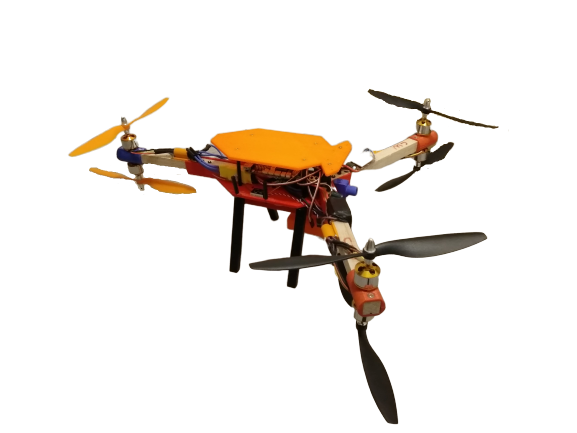
\includegraphics[width=0.8\linewidth]{Y6UAV1-removebg-preview.png}
			\caption{Y6 Hexarotor UAV}
			\label{fig:Y6Hexarotor}
		\end{figure}
		\space
		\section{UAV}
		
			The UAV under consideration throughout this project is an asymmetrical Y6 hexarotor. This kind of configuration has actuators in 3 counter-rotating co-axial pairs and 3 motor groups. A coaxial Y6 hexarotor is mechanically simpler than a classical helicopter since it has propellers with constant pitch and without a swash plate \cite{6}. The advantages of Y6 hexarotors with respect to other multirotor configurations and classical helicopters is that the coaxial configuration increases the thrust without increasing the frame size, while naturally eliminating the loss of efficiency due to direct torque compensation, another advantage of this configuration is better stability. However, the disadvantages are the higher energy consumption for six propulsion units and inefficiency due to the aerodynamic interaction present with co-axial actuator combinations \cite{9}. The UAV is actuated by 6 1000Kv BLDC motors \cite{14}, attached to 6 10x45inch propellers and is powered by a 4-cell lithium-polymer battery. The exact details involved with the design, development and construction of UAVs is beyond the scope of the project investigation but material, mechanical and electronic consideration when designing such craft are explored in \cite{12}.
			
			\begin{figure}[h!]
				\centering
				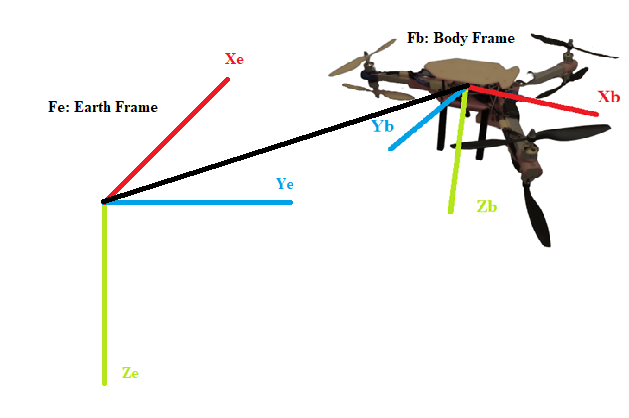
\includegraphics[width=0.7\linewidth]{UAVwithFrames.png}
				\caption{Coordinate Frames}
				\label{fig:Coordinate frames}
			\end{figure} 
		
			Following that, multirotors can be defined as; rigid-bodies free to move in 3-D space with 6-DOF, with all motion restricted to being either rotational or translational.
			\\ \\
			More detailed mathematical models may describe certain multirotor characteristics more accurately, but they also require more computational resources which can lead to, longer simulation times, the inability to successfully complete simulations \cite{5}, and more complex than necessary control design processes and solutions.
			\\ \\
			This project will derive and present 2 models, a non-linear model utilised in simulation, and a Linear model utilised in analysis and control design.
			
		\section{Kinematics}
			
			Multirotor mathematical models have to describe attitude and position according to the geometry of the UAV \cite{6}. one of the most important parts of multirotor modelling is understanding the geometric kinematic relationships between the reference frames \cite{8}. Kinematics is the study of motion in terms of positions and velocities without regard to the forces causing the motion. Multirotor motion can be described by a number of variables called states, that are related and change with suitably chosen axes systems or reference frames \cite{1}. These reference frames are:
				
			\begin{itemize}
				\item
					The Earth Frame: Fe
				\item 
					The Body Frame: Fb  
			\end{itemize}
			\space
			Each frame consists of 3 orthogonal axes, \(Xe,Ye,Ze\) and \(Xb,Yb,Zb\) respectively, about and along which rotational and translational motion respectively can occur. Where Fe is fixed to the earth near the multirotor, such that a flat earth assumption can be made and sustained \cite{2}, and Fb is attached to the vehicle centred at the UAV’s centre of mass, which is free to move with respect to Fe. The usual convention for the axes representation is to have a fixed right-handed axes system with the positive Z axes pointing downwards, towards the earth when level or hovering, the positive X axis pointing forward and the positive y axis pointing towards the right or starboard side. This convention is referred to as the NORTH-EAST-DOWN Right-handed coordinate system \cite{1},\cite{2},\cite{8}. Given the definition of the coordinate reference frames, system variables can now be defined in terms of these reference frames.
			\\ \\
			In Fe, we define vectors:
			\\
			\begin{equation}
				\vec{El} = 
				\begin{bmatrix}
					x \\
					y \\
					z
				\end{bmatrix}
			\end{equation}
			which represent the linear translational positions of Fb’s centre with respect to (w.r.t) Fe.
			\\
			\begin{equation}
				\vec{Er} = 
				\begin{bmatrix}
					\phi \\
					\theta \\
					\psi
				\end{bmatrix}
			\end{equation}
			which represent the angular rotation of Fb about all 3 axes respectively, w.r.t Fe. Which are also known as (roll, pitch, yaw) respectively.
			\\
			In Fb, we define vectors:
			\\
			\begin{equation}
				\vec{Bl} = 
				\begin{bmatrix}
					u \\
					v \\
					w
				\end{bmatrix}
			\end{equation}
			which represents the linear velocity in each Fb axis respectively.
			\\
			\begin{equation}
				\vec{Br} = 
				\begin{bmatrix}
					p \\
					q \\
					r
				\end{bmatrix}
			\end{equation}
			which represents the angular velocity in each Fb axis respectively.
			\\
			From these 12 elemental variables and 4 elemental vectors all, subsequent states and motions can be derived and represented \cite{1},\cite{2},\cite{4}.
			\\ \\
			Using the \(\phi, \theta, \psi\) representation, the rotational motions of Fb w.r.t Fe can be derived by looking at rotations about each axis individually. Decomposing any arbitrary rotation and orientation in 3-D Euclidean space in this manner presents a sequence of three elemental rotations of each axes of Fb w.r.t its counterpart in Fe. These elemental rotation angles are known as $\emph{Euler angles}$  where rotations are represented as direction cosine matrices \cite{1},\cite{2}. These are:
			\\
			\begin{equation}
				R_\psi = 
				\begin{bmatrix}
					C_\psi & S_\psi & 0  \\
					-S_\psi & C_\psi & 0  \\
					0 & 0 & 1
				\end{bmatrix}
			\end{equation}
			\\
			\begin{equation}
				R_\theta = 
				\begin{bmatrix}
					C_\theta & 0 & -S_\theta \\
					0 & 1 & 0 \\
					S_\theta & 0 & C_\theta
				\end{bmatrix}
			\end{equation}
			\\
			\begin{equation}
				R_\phi = 
				\begin{bmatrix}
					1 & 0 & 0 \\
					0 & C_\phi & S_\phi  \\
					0 & -S_\phi & C_\phi
				\end{bmatrix}
			\end{equation}
			\space
			These elemental rotations can by combined via the ZYX convention which multiplies them together in the specific sequence:
			\[R^{-1} = R_\psi \cdot R_\theta \cdot R_\phi\]
			to produce a matrix, the inverse of which, R, is able to map the translational motion of Fb unto Fe given any set of arbitrary \(\phi, \theta, \psi\) values. \cite{1},\cite{2},\cite{3},\cite{4},\cite{5},\cite{6},\cite{7},\cite{8},\cite{9}.
			\\
			\begin{equation}
				R = 
				\begin{bmatrix}
					C_\theta C_\psi & -C_\theta S_\psi + S_\phi S_\theta C_\psi & -S_\phi S_\psi + C_\phi S_\theta C_\psi \\
					C_\theta S_\psi &  C_\phi C_\psi + S_\phi S_\theta S_\psi   & -S_\phi C_\psi + C_\phi S_\theta S_\psi \\
					-S_\theta       &  S_\phi C_\theta                          &  C_\phi C_\theta
				\end{bmatrix}
			\end{equation}
			\\
			Therefore: 
			\[ \dot{\vec{El}} = R \cdot \vec{Bl} \]
			\\
			Which maps the linear velocities and accelerations in Fb to linear velocities and accelerations with respect to Fe.
			\\
			Similarly, to map the angular velocities and accelerations in Fb w.r.t Fe requires another transformation matrix, the inverse of which, T, is also derived from the manipulation of Euler angles \cite{1},\cite{4}. 
			\\
			\begin{equation}
				T = 
				\begin{bmatrix}
					1 & S_\phi T_\theta & C_\phi T_\theta \\
					0 & C_\phi & -S_\phi\\
					0 & \frac{S_\phi}{C_\theta}  & \frac{C_\phi}{C_\theta}
				\end{bmatrix}
			\end{equation} 
			\\
			Therefore:
			\\
			\[\dot{\vec{Er}} = T \cdot \vec{Br} \]
			\\
			Where S, C, T, represent Sin, Cosine and Tan respectively.
				
		\section{Kinetics}
			
			Kinetics is the study of motion considering the forces and torques which cause the motion. As stated in the previous UAV subsection, this investigation looks at a Y6 hexarotor UAV which possesses 6 BLDC motors with propellers in a coaxial motor layout. Each motor propeller unit produces a thrust force, the collective effect of which can be summed and lumped together as a single force F, which means:
			\\
			\[\sum_{i = 1}^{i = 6}F_i\]
			\\
			where i denotes the motor index.
			\\
			Each motor propeller unit or propulsion unit, also produces a reaction torque. When a motor turns, in overcoming air resistance, a reactive force acts on the propeller in the direction opposite to the motor's rotation which produce a torque acting on the UAV body. These torques, $\tau$, can then also be summed together, meaning:
			\\
			\[\sum_{i = 1}^{i = 6}\tau_i\] 
			\\
			The co-axial configuration also ensures single point torque balancing \cite{6}. meaning, so long as all rotors pair each produce the same torque, the net reactive torque produced is zero. The translational and angular motion of the Y6 hexarotor is controlled by thrust forces and torques produced by each motor. The main thrust is the sum of all rotors thrust, and rotational movement is generated by differences in individual motor thrusts and torques \cite{9}.
				
			\subsection{Newton-Euler}
				
				The Multirotor 6-DOF rigid body kinetics takes into account the mass, and the inertia of the body. These are described by differential equations, which are derived through the utilization of the Newton-Euler modelling convention which derives representations of systems dynamics through the application of first principles via newtons 2nd law of motion aggregating all forces and torques applied to the rigid body by its actuators and environment while observing the resultant accelerations produced.
				\\
				Resolving the Forces acting linearly on the UAV produces:
				\\
				\begin{equation}
					M 
					\begin{bmatrix}
						\ddot{x} \\
						\ddot{y} \\
						\ddot{z}
					\end{bmatrix}
					=
					M 
					\begin{bmatrix}
						0 \\
						0 \\
						g
					\end{bmatrix}
					-
					\begin{bmatrix}
						C_\theta C_\psi & -C_\theta S_\psi + S_\phi S_\theta C_\psi & -S_\phi S_\psi + C_\phi S_\theta C_\psi \\
						C_\theta S_\psi &  C_\phi C_\psi + S_\phi S_\theta S_\psi   & -S_\phi C_\psi + C_\phi S_\theta S_\psi \\
						-S_\theta       &  S_\phi C_\theta                          &  C_\phi C_\theta
					\end{bmatrix}
					\begin{bmatrix}
						\ddot{u} \\
						\ddot{v} \\
						\ddot{w} 
					\end{bmatrix}
					-
					\begin{bmatrix}
						D_lxx & 0 & 0 \\
						0 & D_lyy & 0 \\
						0 & 0 & D_lzz
					\end{bmatrix}
					\begin{bmatrix}
						\dot{x} \\
						\dot{y} \\
						\dot{z} 
					\end{bmatrix}
				\end{equation}  
				\[ M \cdot \ddot{\vec{El}} = R \cdot \ddot{\vec{Bl}} - M \cdot \vec{g} - diag(D_l) \cdot \dot{\vec{El}}\] 
				where M is mass, g is acceleration due to gravity acting in the vertical Ze axis plane, and \(D_l\) is a diagonal matrix of drag coefficients with aerodynamic drag acting directly proportional to velocity in the Fe frame.
				\\
				Given that all thrust forces from the motor act along the same Zb axis plane, and there are no other force acting in the other axes therefore, the resultant equation can be rewritten as:
				\\
				\begin{equation}
					M 
					\begin{bmatrix}
						\ddot{x} \\
						\ddot{y} \\
						\ddot{z}
					\end{bmatrix}
					=
					M 
					\begin{bmatrix}
						0 \\
						0 \\
						g
					\end{bmatrix}
					-
					\begin{bmatrix}
						C_\theta C_\psi & -C_\theta S_\psi + S_\phi S_\theta C_\psi & -S_\phi S_\psi + C_\phi S_\theta C_\psi \\
						C_\theta S_\psi &  C_\phi C_\psi + S_\phi S_\theta S_\psi   & -S_\phi C_\psi + C_\phi S_\theta S_\psi \\
						-S_\theta       &  S_\phi C_\theta                          &  C_\phi C_\theta
					\end{bmatrix}
					\begin{bmatrix}
						0 \\
						0 \\
						\sum F_i 
					\end{bmatrix}
					-
					\begin{bmatrix}
						D_lxx & 0 & 0 \\
						0 & D_1yy & 0 \\
						0 & 0 & D_lzz
					\end{bmatrix}
					\begin{bmatrix}
						\dot{x} \\
						\dot{y} \\
						\dot{z} 
					\end{bmatrix}
				\end{equation}  
				Resolving the torques and forces acting angularly on the UAV in Fb produces:
				\\
				\begin{equation}
					\begin{bmatrix}
						Ixx & 0 & 0 \\
						0 & Iyy & 0 \\
						0 & 0 & Izz
					\end{bmatrix} 
					\begin{bmatrix}
						\dot{p} \\
						\dot{q} \\
						\dot{r}
					\end{bmatrix}
					=
					\begin{bmatrix}
						A_p \\
						A_q \\
						A_r
					\end{bmatrix}
					-
					\begin{bmatrix}
						p \\
						q \\
						r 
					\end{bmatrix}
					\times
					\begin{bmatrix}
						Ixx & 0 & 0 \\
						0 & Iyy & 0 \\
						0 & 0 & Iyy
					\end{bmatrix}
					\begin{bmatrix}
						p \\
						q \\
						r 
					\end{bmatrix}
					-
					\begin{bmatrix}
						D_rxx & 0 & 0 \\
						0 & D_ryy & 0 \\
						0 & 0 & D_rzz
					\end{bmatrix}
					\begin{bmatrix}
						p \\
						q \\
						r
					\end{bmatrix}
				\end{equation} 
				\[ I \cdot \dot{\vec{Br}} = A - C -  diag(D_r) \cdot \vec{Br}  \]
				Where A is the vector of torques generated by the sum of motor forces and torques in each axis, C is the Corriolis matrix formed of the cross product between the angular velocity vector and the diagonal inertia Tensor I, and \(D_r\) is the diagonal matrix of drag coefficients acting against motion in each axis.. 
				\\
				The A vector breaks down to:
				\begin{equation}
				 	A_p = L_1 ((F_1+F_2) - (F_3+F_4))
				\end{equation}
				\begin{equation}
				 	A_q = L_2 ((F_1+F_2+F_3+F_4) - L_3 (F_5+F_6)) 
				\end{equation}
				\begin{equation}
					 A_r = \sum_{i = 1}^{i = 6}\tau_i 
				\end{equation}
				Where L is the perpendicular distance from each motor group to the centre of mass.
					
				\subsection{Asymmetry}
					
					\begin{figure}[h!]
						\centering
						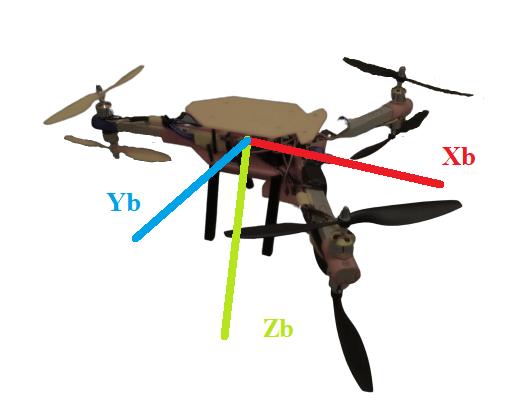
\includegraphics[width=0.6\linewidth]{UAVBodyFrame.png}
						\caption{UAV with Body Frame}
						\label{fig:uavbodyframe}
					\end{figure}
						
					Due to the asymmetry of the Y6 hexarotor, mass is not even distributed across the UAV frame. This creates a particular imbalance of inertia about the centre of mass, which is the centre of all rotation in Fb. This leads to a case where I has off diagonal elements\cite{10}. i.e:
					\\
					$$ 
					\begin{bmatrix}
						Ixx & Ixy & Ixy \\
						Iyx & Iyy & Iyz \\
						Izx & Izy & Izz
					\end{bmatrix}
					$$
					\\
					This creates a situation whereby Fb as shown in Figure 3.3, is inaccurate and instead, is transposed to some other orientation, meaning rotation about the centre mass will occur in an oblong manner.
					\\
					To correct this, it is possible to adjust the inertia tensor by deriving some diagonalising operation such as performing an Eigenvector decomposition \cite{10}, this transformation will then need to be applied to all inertia dependant terms in the angular motion calculation.
					\\  
					However, for the purpose of this investigation, it is possible to operate under the assumption that the system is symmetrical, as presented by a purely diagonal inertial tensor. This is due to the off-diagonal terms in the inertia matrix being far lower in magnitude than the diagonal terms themselves, meaning that the transposed reference frame does not differ too significantly from assumed symmetrical axes, thus any deviations can be reasonably neglected \cite{10}.
			
		\section{Actuator Dynamics}
			
			\begin{figure}[h!]
				\centering
				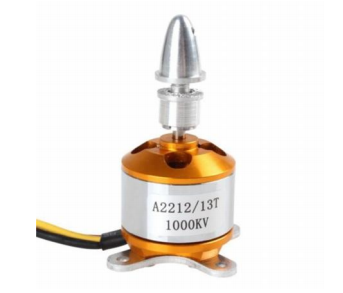
\includegraphics[width=0.5\linewidth]{BLDC.png}
				\caption{A2212/13T 1000KV BLDC Motor}
				\label{fig:BLDC}
			\end{figure}
				
			\begin{figure}[h!]
				\centering
				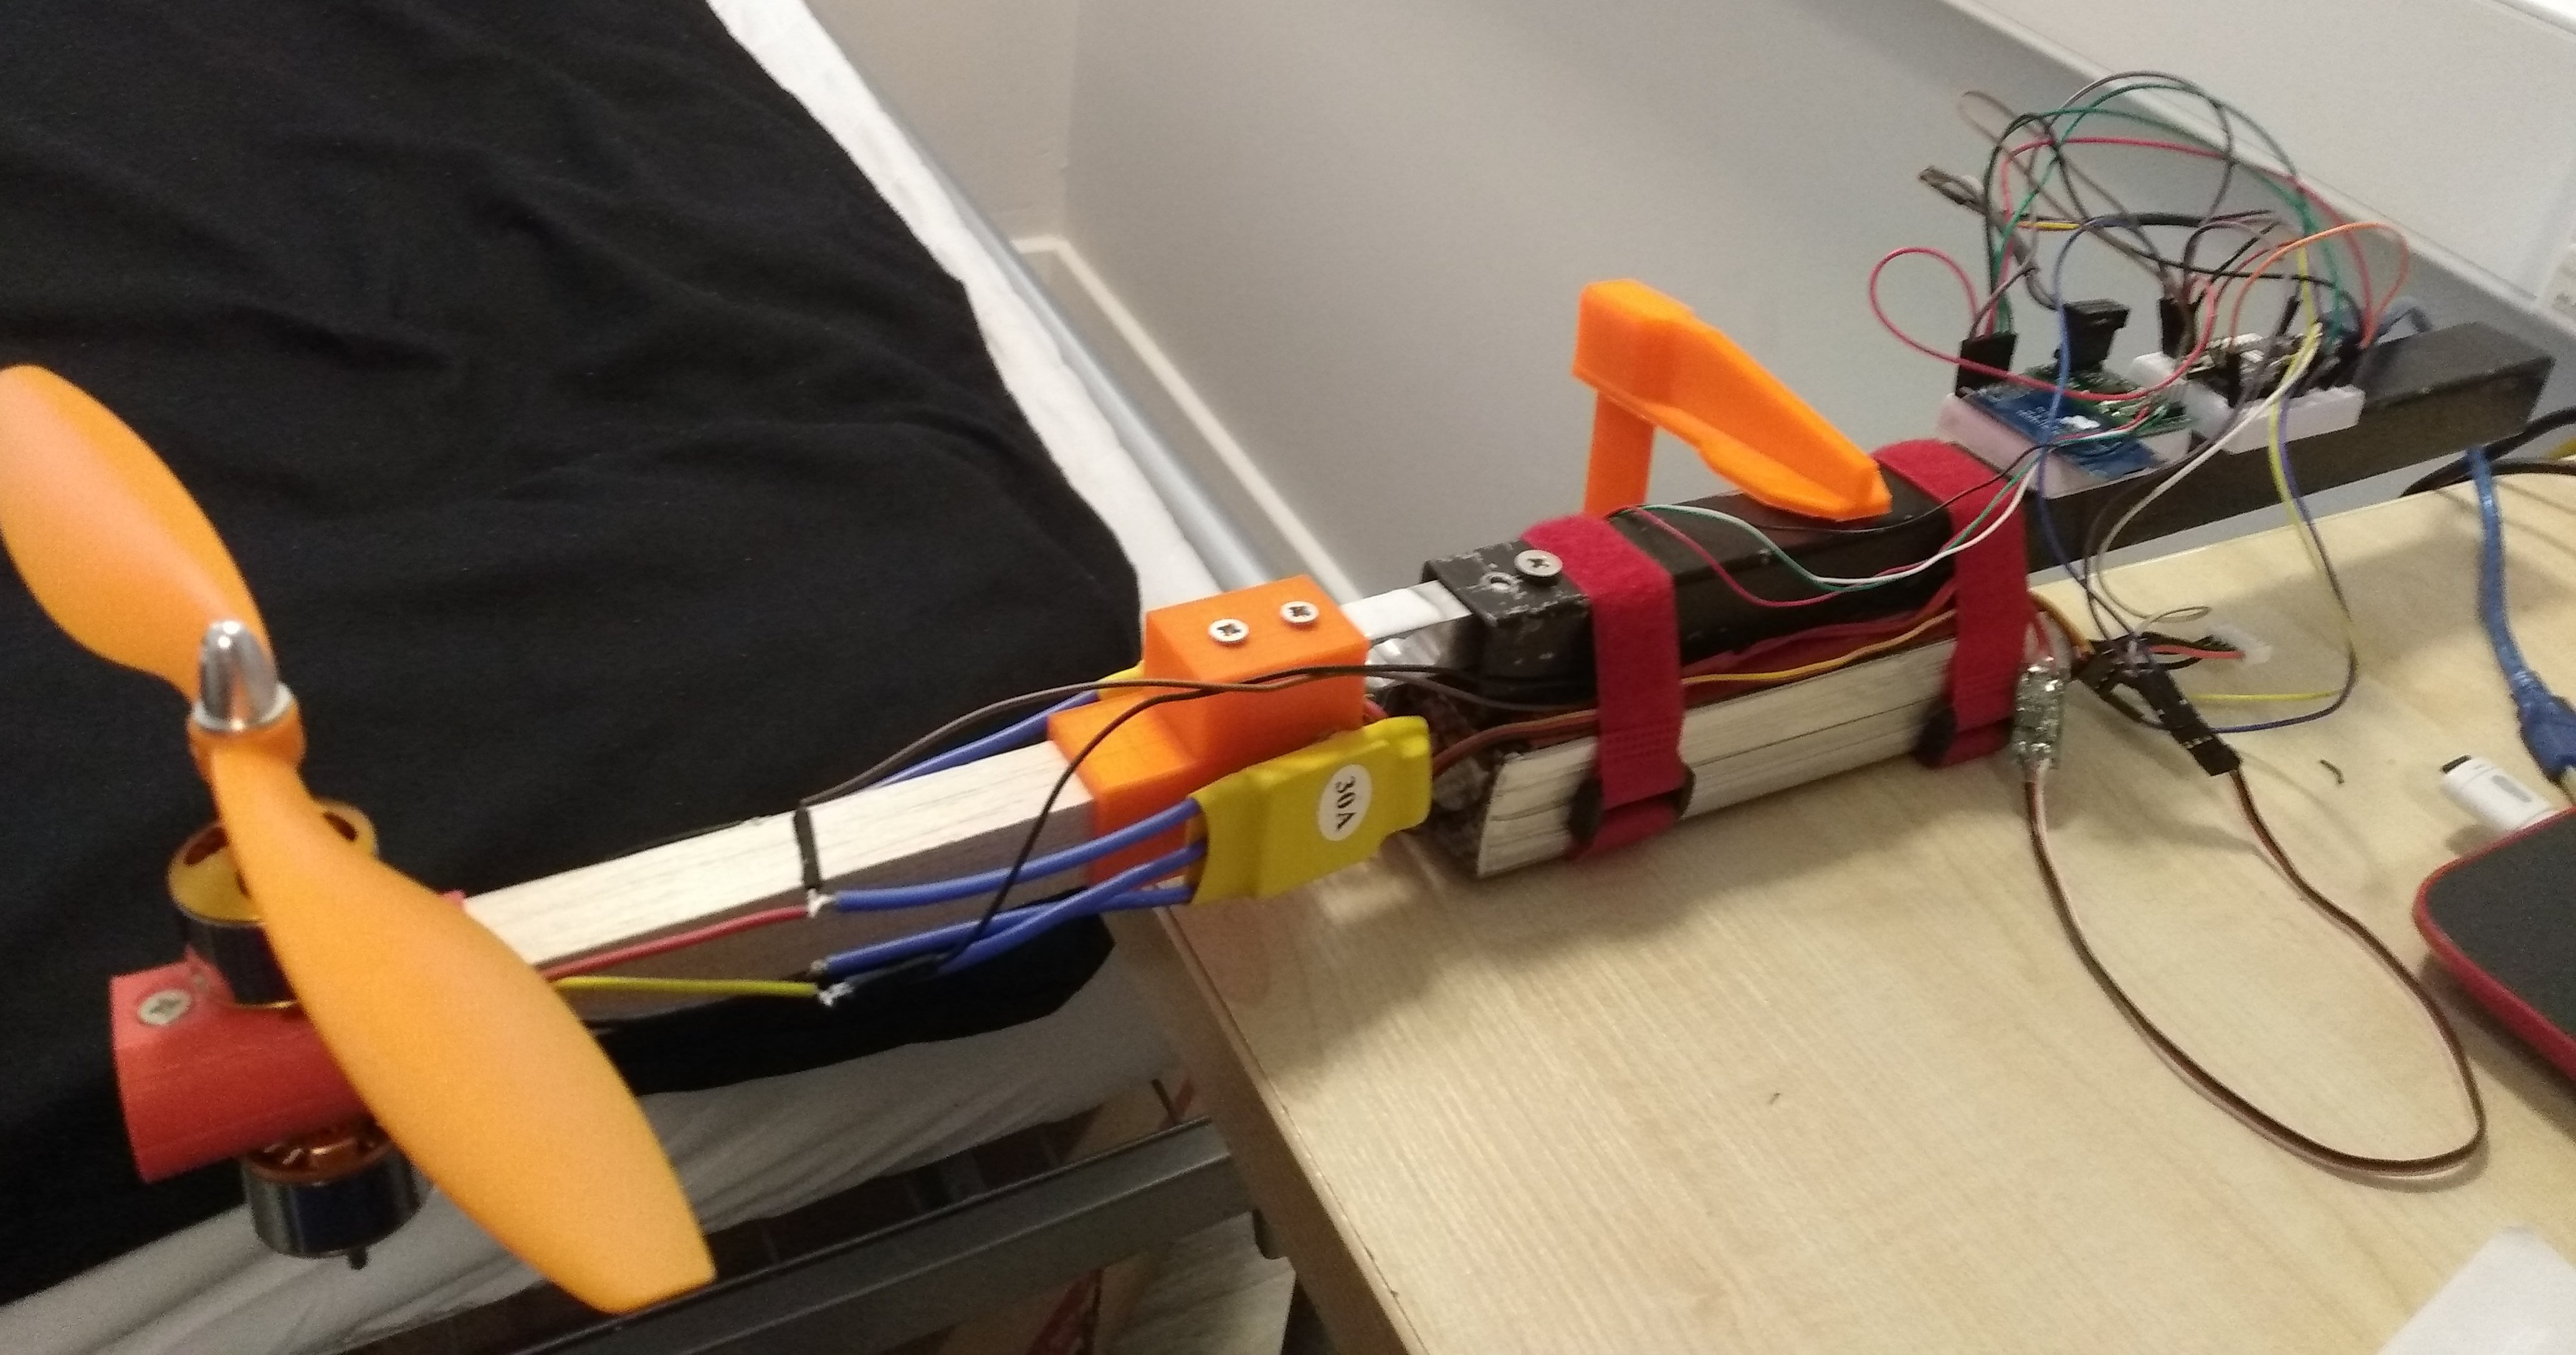
\includegraphics[width=0.7\linewidth]{TestStand1.jpg}
				\caption{Motor Test Stand}
				\label{fig:motorteststand}
			\end{figure}
				
			The thrust forces and torques acting on the multirotor UAV are primarily generated by propulsion units consisting of a BLDC motor, shown in Figure 3.4, an ECS and propeller. In order to produce a useful and fully developed systems model, the characteristics of the propulsion units must be known. This can either be done via first principles analysis looking at the mechanical, electrical and aerodynamic properties of each individual component, before calculating and then applying the results together in series to produce a high order, high fidelity model as is presented in \cite{17}. 
			\\ \\
			However taking this approach in many cases is unnecessary. This is due to being able to derive a lumped parameter model, which views the sum total of all the individual components as a single system with singular dynamics. Therefore, using system response analysis and computational methods such as data fitting, it is possible via experimental systems identification to generate a lower order, minimum realisation model of sufficient fidelity \cite{9},\cite{12},\cite{15},\cite{16}. The systems identification approach involves the derivation of lumped parameter linear input-output models, between input PWM signal widths and the output angular velocity, torque and thrust forces respectively using a motor test stand, shown in Figure 3.5, which consists of a load cell, for measuring forces and torques as well as an electronic revolutions per minute (RPM) sensor.
			\\
			\begin{figure}[h!]
				\centering
				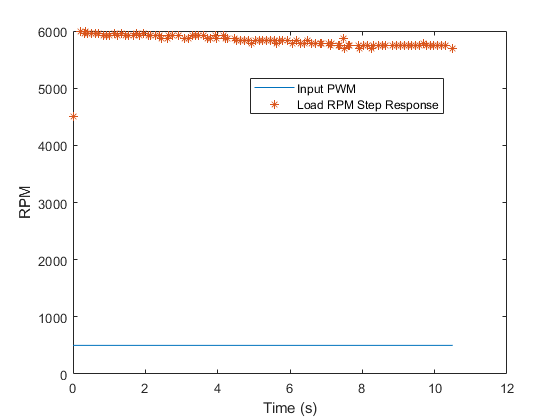
\includegraphics[width=0.7\linewidth]{InputStepData.png}
				\caption{Motor Input Step Data}
				\label{fig:inputstepdata}
			\end{figure}
			\\
			Using the Test stand, input-output PWM to RPM data is collected. Shown in Figure 3.6, is the response of a propulsion unit to a step input of 500$\mu s$. This data was then passed through the MATLAB systems identification application where, in order to account for potential delays in the input response and produce a simple model, a first order transfer function model of the form:
			\\
			\[ \frac{K_u}{\tau_m s + 1} \]
			\\
			was fit to the data, this transfer function can then be reformulated into a differential equation
			\begin{equation}
				\dot{\omega_n} = -\frac{1}{\tau_m}\omega_n	 + \frac{K_u}{\tau_m}\mu_n
			\end{equation}
			Where, $K_u$, is motor gain, $\tau_m$ is the response time constant, $\mu_n$ is the input PWM signal width and $\omega_n$ is the angular velocity. Figure 3.7 shows the response of the identified model to the same step of 500$\mu s$.
			
			\begin{figure}[h!]
				\centering
				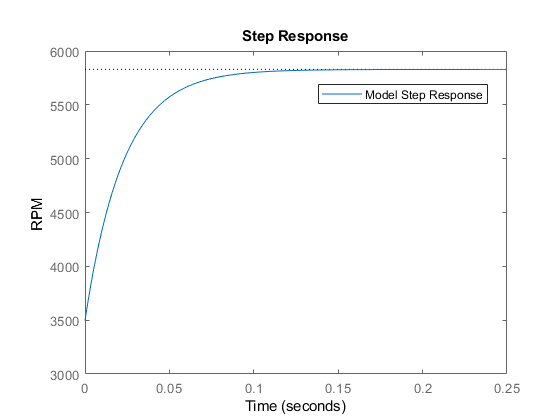
\includegraphics[width=0.7\linewidth]{ModelStep.png}
				\caption{First Order Model Step Response}
				\label{fig:modelstep}
			\end{figure}
			
			It is important to note that due to filtration present in the ESCs, the response time constant is sensitive to the frequency of the input PWM signal, therefore, throughout the investigation a frequency of 400 Hz is maintained. Similarly, using the test stand, as shown in Figures 3.8 and 3.9, data displaying the relationship between the force and torque produced by the propulsion unit against generated angular velocity is shown. 2 quadratic models of the form: 
			\begin{equation}
				F_n = K_a \omega_n^2 + K_b\omega_n
			\end{equation}
			\begin{equation}
				\tau_n = K_\tau \omega_n^2
			\end{equation}
			respectively are then fit to the data where $\omega$ is the angular velocity of the motor, $K_a$, $K_b$ and $K_\tau$ are the force and torque coefficients respectively derived from the quadratic models. Due to the complex aerodynamic interactions from the overlapping air flow between the coaxial pairs, the actual thrust force produced is lower than would be expected from the sum of the two propulsion units \cite{14}. This loss is represented by a gain $K_w$ that is less than 1 and applied to all odd indexed propulsion units.	
			
			\begin{figure}[h!]
				\centering
				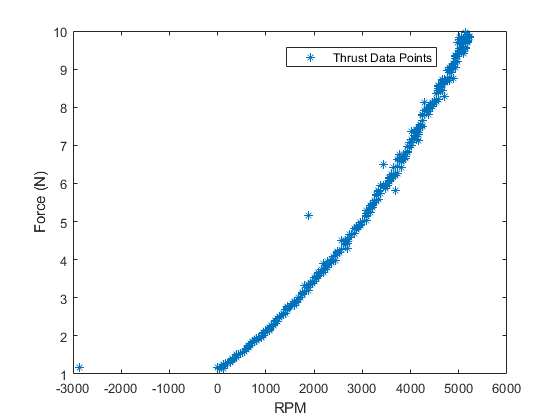
\includegraphics[width=0.7\linewidth]{ThrustData.png}
				\caption{Thrust against RPM}
				\label{fig:thrustdata}
			\end{figure}
			
			\begin{figure}[h!]
				\centering
				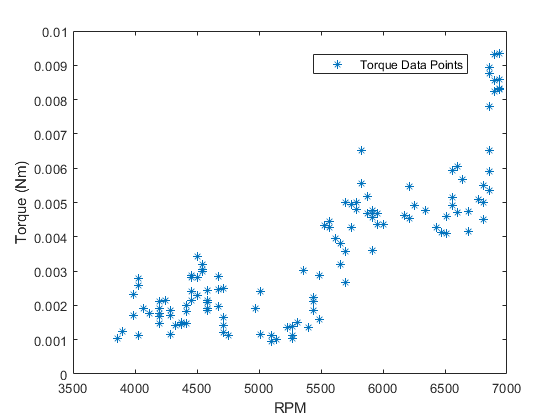
\includegraphics[width=0.7\linewidth]{TorqueData.png}
				\caption{Torque against RPM}
				\label{fig:torquedata}
			\end{figure}
		
		\newpage
			
		\section{Non-Linear Model}
			
			Collating all the derived models process presents the following non-linear mathematical model describing the dynamics of the Y6 hexarotor UAV. which will be used to produce simulations of the system in MATLAB/Simulink.
			\\
			Translational Motion:
			\\ 
			$$ 
				M 
				\begin{bmatrix}
				\ddot{x} \\
				\ddot{y} \\
				\ddot{z}
				\end{bmatrix}
				=
				M 
				\begin{bmatrix}
				0 \\
				0 \\
				g
				\end{bmatrix}
				-
				\begin{bmatrix}
				C_\theta C_\psi & -C_\theta S_\psi + S_\phi S_\theta C_\psi & -S_\phi S_\psi + C_\phi S_\theta C_\psi \\
				C_\theta S_\psi &  C_\phi C_\psi + S_\phi S_\theta S_\psi   & -S_\phi C_\psi + C_\phi S_\theta S_\psi \\
				-S_\theta       &  S_\phi C_\theta                          &  C_\phi C_\theta
				\end{bmatrix}
				\begin{bmatrix}
				0 \\
				0 \\
				\sum F_n 
				\end{bmatrix}
				-
				\begin{bmatrix}
				D_lxx & 0 & 0 \\
				0 & D_1yy & 0 \\
				0 & 0 & D_lzz
				\end{bmatrix}
				\begin{bmatrix}
				\dot{x} \\
				\dot{y} \\
				\dot{z} 
				\end{bmatrix}
			$$ 
			\\
			Rotational Motion:
			\\
			$$ 
				\begin{bmatrix}
				Ixx & 0 & 0 \\
				0 & Iyy & 0 \\
				0 & 0 & Izz
				\end{bmatrix}
				\begin{bmatrix}
				\dot{p} \\
				\dot{q} \\
				\dot{r}
				\end{bmatrix}
				=
				\begin{bmatrix}
				A_p \\
				A_q \\
				A_r
				\end{bmatrix}
				-
				\begin{bmatrix}
				p \\
				q \\
				r 
				\end{bmatrix}
				\times
				\begin{bmatrix}
				Ixx & 0 & 0 \\
				0 & Iyy & 0 \\
				0 & 0 & Iyy
				\end{bmatrix}
				\begin{bmatrix}
				p \\
				q \\
				r 
				\end{bmatrix}
				-
				\begin{bmatrix}
				D_rxx & 0 & 0 \\
				0 & D_ryy & 0 \\
				0 & 0 & D_rzz
				\end{bmatrix}
				\begin{bmatrix}
				p \\
				q \\
				r
				\end{bmatrix}
			$$ 
			\\
			Where:
				\[ A_p = L_1 ((F_1+F_2) - (F_3+F_4)) \]
				\[ A_q = L_2 ((F_1+F_2+F_3+F_4) - L3 (F_5+F_6)) \]
				\[ A_r = \sum_{n = 1}^{n = 6}\tau_n \]
			and motor propulsion unit dynamics are:
				\[\dot{\omega_n} = -\frac{1}{\tau_m}\omega_n	 + \frac{K_u}{\tau_m}\mu_n\]
				\[ F_n = K_a \omega_n^2 + K_b\omega_n \]
				\[\tau_n = K_\tau \omega_n^2 \]
			\\
			Then applying \(\dot{\vec{Er}} = T \cdot \vec{Br} \) to convert angular velocity in Fb to angular velocity w.r.t Fe:
			\\
			$$
				\begin{bmatrix}
				\dot{\phi} \\
				\dot{\theta} \\
				\dot{\psi}
				\end{bmatrix}
				=
				\begin{bmatrix}
				1 & S_\phi T_\theta & C_\phi T_\theta \\
				0 & C_\phi & -S_\phi\\
				0 & \frac{S_\phi}{C_\theta}  & \frac{C_\phi}{C_\theta}
				\end{bmatrix}
				\begin{bmatrix}
				p \\
				q \\
				r 
				\end{bmatrix}
			$$ 
		
		\newpage
		
		\section{Linearisation}
				
			As with the UAV dynamics presented in the previous subsection, the majority of real world systems are non-linear, in that the states of the systems evolve in some fashion that does not satisfy the criteria for linearity. However, the majority of techniques developed over the decades in systems and control theory have been developed for application to and analysis of linear systems. Therefore in order to utilise these techniques in the presence of Non-linearities it is pertinent to devise some means, a least in a limited sense, of operating with Non-linear systems as if they were linear \cite{11}. one means of accomplishing this is through the application of the Jacobian process linearisation of non-linear systems about specific operating or equilibrium points \cite{11},\cite{18}. First however, several assumptions need to be made to reduce the model complexity making it more amicable to linearisation. 
				
			\begin{enumerate}
				\item 
					The UAV is operating in stationary hover conditions
				\item 
					The effects of drag are negligible
				\item 
					Motor dynamics are purely quadratic
			\end{enumerate}

			Under these assumptions:
			\begin{itemize}
				\item
					$\ddot{\vec{Er}} \approx \dot{\vec{Br}} $
				\item
					C, $D_r$, and $D_l$ = 0
			\end{itemize}
			\space
			This reduces the model down to:
			\begin{equation}
				M 
				\begin{bmatrix}
				\ddot{x} \\
				\ddot{y} \\
				\ddot{z}
				\end{bmatrix}
				=
				M 
				\begin{bmatrix}
				0 \\
				0 \\
				g
				\end{bmatrix}
				-
				\begin{bmatrix}
				C_\theta C_\psi & -C_\theta S_\psi + S_\phi S_\theta C_\psi & -S_\phi S_\psi + C_\phi S_\theta C_\psi \\
				C_\theta S_\psi &  C_\phi C_\psi + S_\phi S_\theta S_\psi   & -S_\phi C_\psi + C_\phi S_\theta S_\psi \\
				-S_\theta       &  S_\phi C_\theta                          &  C_\phi C_\theta
				\end{bmatrix}
				\begin{bmatrix}
				0 \\
				0 \\
				\sum F_n 
				\end{bmatrix}
			\end{equation} 
			\begin{equation} 
				\begin{bmatrix}
				Ixx & 0 & 0 \\
				0 & Iyy & 0 \\
				0 & 0 & Izz
				\end{bmatrix}
				\begin{bmatrix}
				\ddot{\phi} \\
				\ddot{\theta} \\
				\ddot{\psi}
				\end{bmatrix}
				=
				\begin{bmatrix}
				L_1 ((F_1+F_2) - (F_3+F_4)) \\
				L_2 ((F_1+F_2+F_3+F_4) - L3 (F_5+F_6)) \\
				\sum_{n = 1}^{n = 6}\tau_n
				\end{bmatrix}
			\end{equation}
			\begin{equation} 
				\dot{\omega_n} = -\frac{1}{\tau_m}\omega_n	 + \frac{K_u}{\tau_m}\mu_n
			\end{equation}
			\begin{equation} 
				F_n = K_a \omega_n^2
			\end{equation}
			\begin{equation} 
				\tau_n = K_\tau \omega_n^2
			\end{equation}
			\\
			Multiplying out the matrices and collecting terms produces 6 distinct 2nd order non-linear Differential, and 1 linear differential equation representing the dynamics of each motor:
			\\
			\begin{equation}
				\ddot{x} = \frac{\sum_{n=1}^{n=6}K_a \omega_n^2}{M}C\phi S\theta C\psi  + \frac{\sum_{n=1}^{n=6}K_a \omega_n^2}{M}S\phi S\psi
			\end{equation}
			\begin{equation}
				\ddot{y} = \frac{\sum_{n=1}^{n=6}K_a \omega_n^2}{M}C\phi S\theta C\psi  - \frac{\sum_{n=1}^{n=6}K_a \omega_n^2}{M}S\phi C\psi
			\end{equation}
			\begin{equation}
				\ddot{z} = g - \frac{\sum_{n=1}^{n=6}K_a \omega_n^2}{M}C\phi C\theta
			\end{equation}
			\begin{equation}
				\ddot{\phi} = \frac{L_1}{Ixx} ((K_a \omega_1^2+K_a \omega_2^2 +) - (K_a \omega_3^2+K_a \omega_4^2))
			\end{equation}
			\begin{equation}
				\ddot{\theta} = \frac{L_2}{Iyy} ((K_a \omega_1^2+K_a \omega_2^2+K_a \omega_3^2+K_a \omega_4^2) - \frac{L3}{Iyy} (K_a \omega_5^2+K_a \omega_6^2))
			\end{equation}
			\begin{equation}
				\ddot{\psi} = \frac{\sum_{n = 1}^{n = 6}K_\tau \omega_n^2}{Izz}
			\end{equation}
			\begin{equation}
				\dot{\omega_n} = -\frac{1}{\tau_m}\omega_n	 + \frac{K_u}{\tau_m}\mu_n
			\end{equation}
			Here we can define the full state vector:
			$$
				X =
				\begin{bmatrix}
					x,\dot{x},y,\dot{y},z,\dot{z},\phi,\dot{\phi},\theta,\dot{\theta},\psi,\dot{\psi},\omega_1,\omega_2,\omega_3,\omega_4,\omega_5,\omega_6
				\end{bmatrix}
			$$
			However for the purposes of this project the full state isn't utilised as feedback control authority in x and y are not required to maintain a stable hover. therefore, a reduced state can be defined: 
			$$
				X =
				\begin{bmatrix}
				z,\dot{z},\phi,\dot{\phi},\theta,\dot{\theta},\psi,\dot{\psi},\omega_1,\omega_2,\omega_3,\omega_4,\omega_5,\omega_6
				\end{bmatrix}
			$$
				
			\subsection{Jacobian Method}
					
				In order to linearise the system equations, equilibrium points must be defined. These are the set of states and input values for which the system is stationary i.e:
					\[\dot{X} = f(X_e,\mu_e) = 0\]
				where f represents the systems dynamics,therefore, the following equilibrium input and state vectors can be defined:
				$$
					X_e = 
					\begin{bmatrix}
						1.5,0,0,0,0,0,0,0,\omega_e1,\omega_e2,\omega_e3,\omega_e4,\omega_e5,\omega_e6
					\end{bmatrix}
				$$
				$$
					\mu_e = 
					\begin{bmatrix}
						\mu_e1,\mu_e2,\mu_e3,\mu_e4,\mu_e5,\mu_e6
					\end{bmatrix}
				$$
				Following this, the system states are redefined in terms of deviations from these equilibrium points:
					\[\bar{X} = X - X_e\] 
					\[\bar{\mu} = \mu - \mu_e\] 
				These deviation variables are then substituted back into the dynamics equations and a first order Taylor's series expansion is performed. where:
				\begin{equation}
					\dot{\bar{X}} = f(\bar{X},\bar{\mu}) + \frac{\partial f}{\partial X}\bigg\vert_{\mu = \mu_e}^{X = X_e} + \frac{\partial f}{\partial \mu}\bigg\vert_{\mu = \mu_e}^{X = X_e}
				\end{equation}
				and:
					\[ f(\bar{X},\bar{\mu}) = 0 \]
				These differential equations approximately govern the deviation variables, and as long as they remain small, this presents a linear, time-invariant, differential equation, as the derivatives of $\bar{X}$ are now linear combinations of the deviation states and the deviation inputs, $\bar{\mu}$ \cite{11}. 
				\\
				Finally, the Linear Continuous-Time State-Space model emerges following:
				\\
				\begin{equation}
					A = \frac{\partial f}{\partial X}\bigg\vert_{\mu = \mu_e}^{X = X_e}, \in R ^{n\times n}
				\end{equation}
				\\
				\begin{equation}
					B = \frac{\partial f}{\partial \mu}\bigg\vert_{\mu = \mu_e}^{X = X_e} , \in R ^{n\times m}
				\end{equation} 
				Where n is the number of states, m the number of inputs, A the n-by-n dynamics matrix and B the n-by-m input matrix.
				\\ \\
				Thus:
				\\
				\setcounter{MaxMatrixCols}{15}
				A = 
				\begin{equation}
					\begin{bmatrix}
						0&1&0&0&0&0&0&0&0&0&0&0&0&0\\
						0&0&0&0&0&0&0&0&\frac{2K_a\omega_e1}{M}&\frac{2K_wK_a\omega_e2}{M}&\frac{2K_a\omega_e3}{M}&\frac{2K_wK_a\omega_e4}{M}&\frac{2K_wK_a\omega_e5}{M}&\frac{2K_wK_a\omega_e6}{M}\\
						0&0&0&1&0&0&0&0&0&0&0&0&0&0\\
						0&0&0&0&0&0&0&0&\frac{2L_1K_a\omega_e1}{Ixx}&\frac{2L_1K_wK_a\omega_e2}{Ixx}& \frac{-2L_1K_a\omega_e3}{Ixx}&\frac{-2L_1K_wK_a\omega_e4}{Ixx}&0&0\\
						0&0&0&0&0&1&0&0&0&0&0&0&0&0\\
						0&0&0&0&0&0&0&0&\frac{2L_1K_a*\omega_e}{Iyy}&\frac{2L_2K_wK_a\omega_e2}{Iyy}& \frac{2L_2K_a\omega_e3}{Iyy}&\frac{2L_2K_wK_a\omega_4}{Iyy}&\frac{-2L_3K_a*\omega_e5}{Iyy}&\frac{-2L_3K_wK_a\omega_e6}{Iyy}\\
						0&0&0&0&0&0&0&1&0&0&0&0&0&0\\
						0&0&0&0&0&0&0&0&\frac{-2K_\tau\omega_e1}{Izz}&\frac{2K_\tau\omega_e2}{Izz}&\frac{2K_\tau\omega_e3}{Izz}&\frac{-2K_\tau\omega_e4}{Izz}&\frac{-2K_\tau\omega_e5}{Izz}&\frac{2K_\tau\omega_e6}{Izz}\\
						0&0&0&0&0&0&0&0&\frac{-1}{\tau_m}&0&0&0&0&0\\
						0&0&0&0&0&0&0&0&0&\frac{-1}{\tau_m}&0&0&0&0\\
						0&0&0&0&0&0&0&0&0&0&\frac{-1}{\tau_m}&0&0&0\\
						0&0&0&0&0&0&0&0&0&0&0&\frac{-1}{\tau_m}&0&0\\
						0&0&0&0&0&0&0&0&0&0&0&0&\frac{-1}{\tau_m}&0\\
						0&0&0&0&0&0&0&0&0&0&0&0&0&\frac{-1}{\tau_m}
					\end{bmatrix}
				\end{equation}
				\\
				B = 
				\begin{equation}
					\begin{bmatrix}
					0&0&0&0&0&0\\
					0&0&0&0&0&0\\
					0&0&0&0&0&0\\
					0&0&0&0&0&0\\
					0&0&0&0&0&0\\
					0&0&0&0&0&0\\
					0&0&0&0&0&0\\
					0&0&0&0&0&0\\
					\frac{K_u}{\tau_m}&0&0&0&0&0\\
					0&\frac{K_u}{\tau_m}&0&0&0&0\\
					0&0&\frac{K_u}{\tau_m}&0&0&0\\
					0&0&0&\frac{K_u}{\tau_m}&0&0\\
					0&0&0&0&\frac{K_u}{\tau_m}&0\\
					0&0&0&0&0&\frac{K_u}{\tau_m}
					\end{bmatrix}
				\end{equation}
				Where $n = 14$ and $m = 6$.
			
			\section{Summary}
				
				This Chapter:
				\begin{itemize}
					\item 
				 		Introduced and defined the UAV system under consideration.
				 	\item 
				 		Discussed and derived the mathematical equations describing the non-linear behaviour of the UAV, using both the kinematics and kinetics representations while implementing Euler angles, the Newton-Euler convention, and describing their relevance to modelling. 
				 	\item
				 		Presented a means by which, through experimental identification, the key parameters that define the actuation forces may be derived, and discussed the relevance of mass distribution considerations.
				 	\item
				 		Presented a means of converting the derived non-linear dynamics into a form which could be utilised in the development of linear control systems, then developed and presented said linearised model.
				\end{itemize}
			 
			\newpage
			
			\begin{table}[h!]
			\centering
			\begin{tabular}{ |p{1.5cm}||p{9.5cm}|p{5cm}|  }
				\hline
				\multicolumn{3}{|c|}{Model Parameters} \\
				\hline
				Character& Name  & Value  \\
				\hline
				M        &  Mass                                                 & 1.455882 Kg\\
				Ixx      &  Inertia about Xb                                     & 0.014 $N/m^2$\\
				Iyy      &  Inertia about Yb                                     & 0.028 $N/m^2$\\
				Izz      &  Inertia about Zb                                     & 0.038 $N/m^2$\\
				$D_lxx$  &  Translational Drag Coefficient in Xe                 & 0.01212\\
				$D_lyy$  &  Translational Drag Coefficient in Ye                 & 0.01212\\
				$D_lzz$  &  Translational Drag Coefficient in Ze                 & 0.0648\\
				$D_rxx$  &  Angular Drag Coefficient in Xb                       & 0\\
				$D_ryy$  &  Angular Drag Coefficient in Yb                       & 0\\
				$D_rzz$  &  Angular Drag Coefficient in Zb                       & 0\\
				$L_1$    &  Lateral Length From Motor 1 To Center Of Mass        & 0.19 m\\
				$L_2$    &  Longitudinal Length From Motor 1 To Center Of Mass   & 0.18 m\\
				$L_3$    &  Longitudinal Length From Motor 5 To Center Of Mass   & 0.30 m\\
				$K_u$    &  Motor RPM Gain                                       & $515.5 \times \tau_m$\\
				$\tau_m$ &  Motor RPM Time Constant                              & $\frac{1}{44.22}$\\
				$K_w$    &  Quadratic RPM to Force Gain                          & 0.85\\
				$K_a$    &  Quadratic RPM to Force Gain                          & 1.812e-07\\
				$K_b$    &  Linear RPM to Force Gain                             & 0.0007326\\
				$K_\tau$ &  Quadratic RPM to Torque Gain                         & 7.708e-10\\
				$g$      & Acceleration Due To Gravity                           & 9.81 $m/s^2$\\
				\hline
			\end{tabular}
			\caption{Table of Model Parameters}
			\label{table:modelparameters}
			\end{table}
			
			\newpage
			
	\chapter{Linear Quadratic Gaussian and Model Predictive Control}
		
		\section{Introduction}
		
			The objective of this investigation is to devise control systems capable of taking the UAV to a state of stable hovering conditions. The purpose of designing and implementing control systems is to reject or minimise the effects of disturbance to the system, as well as change the characteristics of the system so as to meet performance requirements. Therefore in order to accomplish this with the UAV model derived in chapter 3, this investigation seeks to develop both LQG and an LQ-MPC control systems. These are both advanced linear model based controller that are extremely powerful and are able to nominally provide stability guarantees with wide margins. In order to develop and then implement these the following themes will be explored:
		 
			\begin{enumerate}
				\item 
					Discretization
				\item 
					Model Analysis
				\item 
					LQG
				\item
					LQ-MPC
			\end{enumerate}
		
		\section{Discretization}
		
			The Linearised model obtained in chapter 3 is derived in the continuous-time domain. In order to design control systems which can be implemented unto a digital embedded microprocessor, the control laws must be in discrete-time domain.
			\\
			This can be done either by designing the control systems in the continuous-time domain then converting the resulting continuous control laws into discrete ones, or by transforming the entire continuous-time model to the discrete-time domain then designing the control laws using the discrete-time system model \cite{18}. This investigation utilises the latter method.
			\\
			To convert a continuous-time state space model of form:
			\[
				\dot{X(t)} = AX(t) + B\mu(t)
			\]
			to the discrete-time domain Produces:
			\begin{equation}
				X(k+1) = A_{dt}X(k) + B_{dt}\mu(k)
			\end{equation}
			where:
			\begin{equation}
				A_{dt} = e^{AT} 
			\end{equation}
			\begin{equation}
				B_{dt} = A^{-1}(e^{AT} - I)B
			\end{equation}
			\space
			and T is the discretization sample time, k is the time increment, and I an identity matrix of sufficient dimension.
			
		\section{Model Analysis}
			
			Model-Based feedback control systems design utilises insights gained from having the system model on hand to inform the design process and determine how best adjustments should be made. In order to accomplish this, the system is first thoroughly analysed and understood. Given the linear state state-space model developed at the end of chapter 3, the discretization performed in previous section, along with the values presented in the Table 3.1, it is possible to use linear system analysis techniques to arrive at key insight such as:
			
			\begin{itemize}
				\item 
					Stability
				\item 
					Reachability
				\item
					Observability
			\end{itemize}
		
			\subsection{Stability}
			
				\begin{figure}[h!]
					\centering
					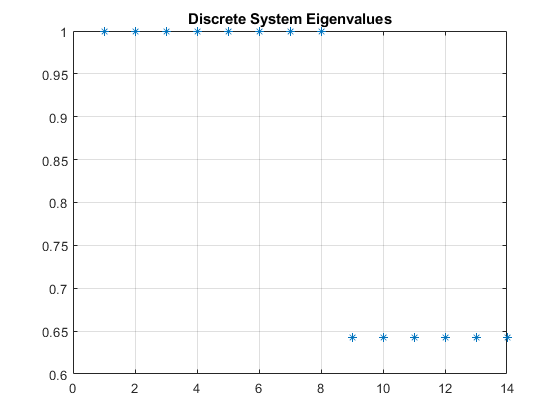
\includegraphics[width=0.8\linewidth]{DiscreteSystemPoles.png}
					\caption{Open-Loop Eigenvalues}
					\label{fig:openloopeigenvalues}
				\end{figure}
			
				Stability theory plays a key role in the design of control. There are different kinds of stability problems that arise in the study of dynamical systems. The stability of systems about equilibrium operating points is usually characterised in the Lyapunov sense where an equilibrium point is said to be stable where all solutions starting nearby the equilibrium points stay nearby for all time, otherwise the system is said to be unstable \cite{13},\cite{18}. 
				\\
				This definition of stability can be further specified to define stability in the asymptotic sense, where a system is said to be asymptotically stable if all solutions starting nearby the equilibrium points not only stay nearby, but also tend to the equilibrium point as time goes to infinity \cite{13},\cite{18}.
				\\
				For linear state-space systems, stability can be assertained from the locations of the eigenvalues, $\lambda$, of the $A_{dt}$ matrix, This process is know as Lyapunov's indirect method \cite{13} where:
				
				\begin{equation}
					det|A_{dt} - \lambda I| = 0
				\end{equation}
				\space
				Figure 4.1 reveals the presence 6 eigenvalues with a value less than 1, and 8 eigenvalues with a value of 1. For discrete-time systems, stability can be said to be asymptotic if all eigenvalues are strictly within the unit circle, Lyapunov if all eigenvalues are within or on the unit circle, and unstable otherwise \cite{13},\cite{18}. Therefore the linear systems model can be said to be stable in the sense of Lyapunov. This implies also that the non-linear systems model is locally stable in the sense of Lyapunov about the equilibrium points $X_e$ \cite{13}.
				\\
				However due to real world disturbances such as model uncertainty, sensor noise and external wind disturbances, the system will not remain at the point of equilibrium save for the intervention of some control law to reject the effect of these disturbances. Hence, the system, although statically stable, is dynamically unstable.
				
			\subsection{Reachability}
				
				Reachability is a property which is determined by coupling the inputs into the system and the states, a system is said to reachable if for any initial set of state values $X_0$, and any final set of state value, $X_f$, there is a control signal $\mu(k)$ that can take the system from $X_0$ at k = 0, to  $X_f$ with some finite time \cite{18},\cite{25}.
				\\
				A system is said to be reachable if the reachability matrix:
				\begin{equation}
					W_r = 
					\begin{bmatrix}
						B_{dt} & A_{dt}B_{dt} & \dots & A_{dt}^{n-1}B_{dt}
					\end{bmatrix}
				\end{equation}
				is full rank equalling the number of state, n.
				\\
				Thus, as the rank of $W_r$ is equals to n, the system can be said to be reachable. 
				\\
				The less stringent property of stabilisability can also be defined where only the unstable states need be reachable.
				
			\subsection{Observability}
				
				Like reachability, Observability is a property which is determined by coupling, in this case, that between the system outputs and the system states. Therefore the system outputs, $Y$, must be defined where $Y$ is a subset of the state $X$ :
				\[
					Y \in X
				\]
				where:
				\begin{equation}
					Y = [z,\phi,\theta,\psi]
				\end{equation}
				Therefore, a matrix to perform the state selection is defined as:
				\\
				\begin{equation}
					Y(k) = CX(k)  
				\end{equation}
				\[
					C \in R^{p \times n}  
				\]
				where p is the number of outputs.
				\\
				Thus we define:
				\setcounter{MaxMatrixCols}{15}
				\begin{equation}
					C =
					\begin{bmatrix}
						1&0&0&0&0&0&0&0&0&0&0&0&0&0 \\
						0&0&1&0&0&0&0&0&0&0&0&0&0&0 \\
						0&0&0&0&1&0&0&0&0&0&0&0&0&0 \\
						0&0&0&0&0&0&1&0&0&0&0&0&0&0
					\end{bmatrix}  
				\end{equation}
				\[
					p = 4  
				\]
				where:
				\[
					C_{dt} = C
				\]
				A system is said to observable if for all time, it is possible to, from a limited set of state measurements $Y(k)$, and knowledge of the inputs $\mu(k)$, to \emph{uniquely} obtain the full state, X(k) \cite{18}.
				\\
				A system is said to be observable if the observability matrix:
				\begin{equation}
					W_o = 
					\begin{bmatrix}
						C_{dt}\\
						C_{dt}A_{dt}\\ 
						\vdots \\
						C_{dt}A_{dt}^{n-1}
					\end{bmatrix}
				\end{equation}
				is full rank equalling n.
				\\
				Again as with reachability, a less stringent property, detectability, can also be defined where only the unstable states need be observable.
				\\ \\
				Interestingly, for this combination of dynamics $A_{dt}$ and $C_{dt}$, it is found that the $W_0$ is not full rank, and therefore the system in its current form is not observable. Upon further analysis, it is discovered that this is as a result of a phenomenon created due to the Coaxial propulsion unit configuration, as there are numerous combinations of thrust force values that each individual propulsion unit can generate which produce the same resultant torque about the centre of mass making it impossible to obtain a unique full state. One possible solution is to modify the UAV design to include RPM sensors to measure at least 2 non-coaxial motors. However, in the upcoming LQG section, a more elegant solution is proposed.
		
		\section{LQG}
		
			\subsection{Full-State Feedback}
			
				Given a discrete-time linear state-space model of form:
				
				\[X(k+1) = A_{dt}X(k) + B_{dt} \mu(k)\]
				\begin{equation}
					Y(k) = C_{dt} X(k)
				\end{equation}
				\space
				Full-state feedback is a control technique which makes use of the full-state, $X(k)$ of a system, to modify the system's eigenvalue so as to change its characteristic responses\cite{18}. This is done by determining some set of gains $K$ which when applied to the system states, the resultant of which being fed back into the system as inputs, adjust the dynamics of the system, where:
				
				\begin{equation}
					\mu(k) = -K X(k)
				\end{equation}
				
				This leads to a modified closed loop system:
				
				\begin{equation}
					X(k+1) = (A_{dt}-B_{dt}K) X(k)
				\end{equation}
				
				Where the eigenvalue are now determined by:
				
				\begin{equation}
					det|(A_{dt}-B_{dt}K) - \lambda I| = 0
				\end{equation}
				
			\subsection{LQR}
				
				LQR is a technique for finding the set of gains K, in a manner which is in some wise optimal \cite{18},\cite{19},\cite{20},\cite{25}. In order to accomplish this, LQR seeks to find a control sequence \emph{\emph{$\mu$}} to minimise a \emph{quadratic} cost function by formulating the control problem as optimisation problem \(P_\infty(X(0))\), where :
				
				\(P_\infty(X(0)) = \)				
				\begin{equation}
					min_\mu  V_\infty(X(0),\emph{\emph{$\mu$}}) = \sum_{k = 0}^{k = \infty} X^{T} Q X + \mu^{T} R \mu
				\end{equation}
				\(s.t\)
				\[
					X(k+1) = A_{dt}X(k) + B_{dt} \mu(k) , k=1,2,3\dots
				\]
				Where $Q^{n \times n}$, and $R^{m \times m}$, are 2-norm weighing matrices on the states and inputs respectively. These weight are selected via trial and error.
				\\
				Such an optimisation over an infinite horizon, as \(k \to \infty \), would be intractable, however through the application of the Dynamic Programming (DP) formulated from Bellman's principle of optimality, the solution emerges as a result of the derivation of a set of Discrete Algebraic Riccati Equation (DARE) \cite{25} where:
				
				\(DARE = \)
				\[
					K = - (R + B_{dt}^{T} \Pi B_{dt})^{-1} B_{dt}^{T} \Pi A_{dt}
				\]
				\begin{equation}
					\Pi = Q + A_{dt}^{T} A_{dt} - A_{dt}^{T} \Pi B_{dt}(R + B_{dt}^{T} \Pi B_{dt})^{-1} B_{dt}^{T} \Pi A_{dt}
				\end{equation}
				\\
				In order for the optimisation problem to be feasible, certain criteria must be satisfied \cite{18},\cite{25}:
				
				\begin{itemize}
					\item
						Q be at least Positive Semi-definite (P.S.D) and R be strictly Positive Definite (P.D).
					\item
						\( (A_{dt},B_{dt}) \) must be at least stabilisable.
					\item
						\( (C_{dt},A_{dt}) \) must be at least detectable.
				\end{itemize} 
			
			\subsection{Reference Tracking and Integral Action}
				
				The control problem as set up in the previous LQR subsection is one capable of realising a control system with the goal of driving all system states to the equilibrium points. However, in order for the control system to be usefully implemented on a UAV, it must be able to track and set the system outputs $Y$ to, a desired reference target, \emph{\emph{r}}, preferably with no errors asymptotically.
				\\
				Therefore, to accomplish this, the system's model must be augmented to include behaviour which seeks to minimise errors between a reference target and UAV output, this is done through the addition of integration states. hence:
				
				\begin{equation}
					X_{aug} = 
					\begin{bmatrix}
						X \\
						X_I
					\end{bmatrix}
				\end{equation}
				
				Where 	\(X_I = \emph{\emph{r}} - Y \):
				\begin{equation}
					X_I =
					\begin{bmatrix}
						Z_I \\
						\phi_I\\
						\theta_I\\
						\psi_I
					\end{bmatrix}
				\end{equation}
				
				This Leads to augmented discrete state-space Matrices:
				\\
				\begin{equation}
					A_{aug} =
					\begin{bmatrix}
						A_{dt} & \emph{\emph{0}} \\
						-C_{dt}A_{dt} & I
					\end{bmatrix}
					,
					B_{aug} =
					\begin{bmatrix}
						B_{dt}\\
						-C_{dt}B_{dt}
					\end{bmatrix}
					,
					C_{aug} =
					\begin{bmatrix}
						C_{dt} & \emph{\emph{0}}
					\end{bmatrix}
				\end{equation}
				\\   
				Where \emph{\emph{0}} is a square zeros matrix of dimension P and I is an identity matrix of dimension p.
				\\
				Solving the LQR optimisation problem with, $A_{aug}$,$B_{aug}$,$C_{aug}$ and $Q^{n+p \times n+p}$, given this augmented system, produces a control law \cite{19}: 
				
				\begin{equation}
					\mu(k) = - K X(k) + K_I X_I(k)
				\end{equation}
				
				Where:
				
				\begin{equation}
					X_{aug}(k+1) = (A_{aug} - B_{aug}K_{y}) X_{aug}(k) + B_{aug}K_I \emph{\emph{r}}(k)
				\end{equation}
				\[
					K_{y} =
					\begin{bmatrix}
						K & -K_{I}
					\end{bmatrix}
				\]
				\\
				This is implemented in the MATLAB-Simulink environment while taking into account the SBC dynamics such the effects of quantisation from digital to analog and visa-versa conversions which are always present when digital controllers that interface with real analogue continuous-time systems:
				\\
				\begin{figure}[h!]
					\centering
					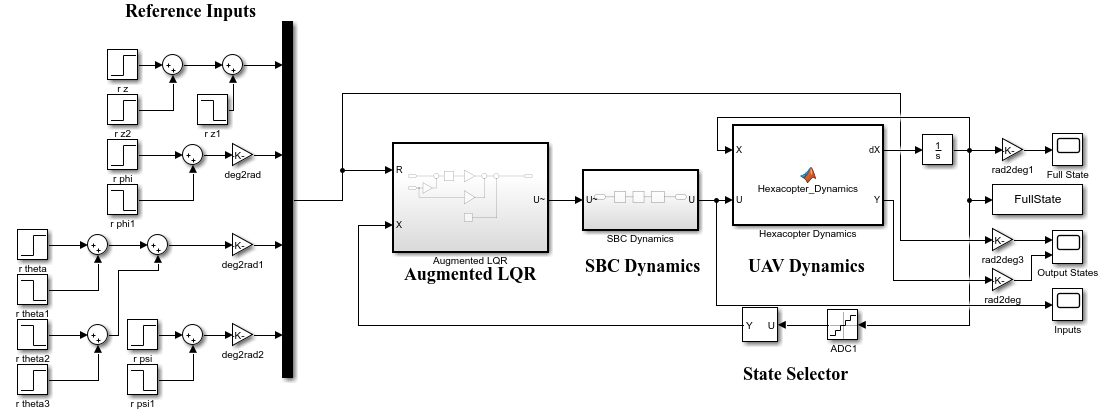
\includegraphics[width=1\linewidth]{LQRSimulink.png}
					\caption{LQR Simulink Implimentation}
					\label{fig:lqrsimulinkimplimentation}
				\end{figure}
				
			\subsection{State Estimation}
			
				The control law devised in LQR subsection was produced under the assumption that the full state of the system, X, is available for full-state feedback, however, this is not the case as only a limited number of state measurements are available and these form the measured outputs, Y. Therefore, in order to utilise a full-state feedback control law, the full-state of the system must be estimated from these limited measurements present. This is performed through the implementation of a State Observer/Estimator. State estimators accomplish this by applying knowledge of the system dynamics through the utilisation of the system's model and its observability property \cite{18},\cite{21},\cite{22},\cite{23},\cite{24}.
				\\ \\
				The estimator mimics the system dynamics giving: 
				\[
					\hat{X}(k+1) = A_{dt}\hat{X} + B_{dt} \mu(k) + L e
				\]
				\begin{equation}
					\hat{Y}(k) = C_{dt}\hat{X}
				\end{equation}
				\\
				where $\hat{X}$ and $\hat{Y}$ are the estimated system states and outputs, L is the estimator gain with e being the output error, which is the difference between the estimator model and the system outputs.
				\[
					e = Y - \hat{Y}
				\]
				As with the systems model, the behaviour of estimator model and thus the quality of the estimation is determined by the state estimation error dynamics \cite{18}, where:
				\[
					\hat{X_e} = X - \hat{X}
				\]
				The open-loop estimator dynamics are given by:
				\begin{equation}
					\hat{X_e}(k+1) = A_{dt}(X - \hat{X})
				\end{equation}
				\\
				with implementation of the observer gain $L$, the closed-loop estimator dynamics are give by:
				\begin{equation}
					\hat{X_e}(k+1) = (A_{dt} - L C_{dt})\hat{X_e}
				\end{equation}
				\\
				If the eigenvalues of the estimator exist outside the unit circle, then the estimator is unstable and the state estimation is be divergent, and if the system is observable, then it is always possible to derive some gain L, to produce any set of desired eigenvalues \cite{18} 
				\\
			\subsection{Estimator Modification}
			
				In the earlier observability subsection, it was found that the system is not observable due to propulsion unit configuration, and the emergent thrust and torque combinations making the estimation of a unique full state impossible.
				\\
				This can be rectified simply be making the system observable by modifying the hardware and measuring the value of some of the motor states via RPM sensors.
				\\
				However, there is another way this can be solved without the need to obtain additional sensors, that is, by virtually augmenting the output, Y to include terms for at least 2 non coaxial motor pairs, then returning an error vector, e ,where the error value for those 2 motors is 0,  therefore:
				
				\setcounter{MaxMatrixCols}{15}
				\begin{equation}
					C_y =
					\begin{bmatrix}
						1&0&0&0&0&0&0&0&0&0&0&0&0&0 \\
						0&0&1&0&0&0&0&0&0&0&0&0&0&0 \\
						0&0&0&0&1&0&0&0&0&0&0&0&0&0 \\
						0&0&0&0&0&0&1&0&0&0&0&0&0&0 \\
						0&0&0&0&0&0&0&0&1&0&0&0&0&0 \\
						0&0&0&0&0&0&0&0&0&0&0&1&0&0 \\
					\end{bmatrix}  
					,
					Y_y =
					\begin{bmatrix}
						Z \\
						\phi\\
						\theta\\
						\psi\\
						\omega_1\\
						\omega_4
					\end{bmatrix}
					,
					e =
					\begin{bmatrix}
						e_1 \\
						e_2\\
						e_3\\
						e_4\\
						0\\
						0
					\end{bmatrix}
				\end{equation}
				\\
				This augmentation has the effect of using the model to completely determine the value of the motor angular velocity by assuming the model is a perfect representation of the actual system. This augmentation is done solely for the purpose of state estimation so there are still only 4 reference input to the controller and only 4 measured outputs, but with this, the system is now fully observable.
				
			\subsection*{The Kalman Filter}
				
				Kalman Filtering encompasses a series of techniques for obtaining an estimator gain L, which is in some wise optimal. This is accomplished by constructing an optimisation problem with the objective of minimising a set of noise measurement covariances which arise from disturbances to the system such those due to model uncertainty and noise present in the output sensor readings, these sources of noise are modelled as Gaussian noise distributions. Thus, when used in combination with the LQR, the combination is called the Linear Quadratic Gaussian.  
				\\
				The Kalman Filter problem is a corollary problem to the LQR, where optimisation is also performed over infinite horizon, requiring the application of DP, and is thus derived resulting in another DARE \cite{18},\cite{21}.
				\\
				There are 2 major implementations of the Kalman filter which are popularly employed.
					
				\begin{itemize}
					\item 
						The Linear Kalman Filter (LKF)
					\item 
						The Extended Kalman Filter (EKF)
				\end{itemize} 
				\space
				The process described above only fully pertains to the design of an LKF. The EKF is used in estimating the states of non-linear systems, utilising the non-linear system model directly but then implementing an online lineariser that linearises the system at each time interval, k, to produce a linear model which is then used to solve for the estimator gain L as stated above \cite{21},\cite{22},[243].
				\\
				However, through experimentation with the estimator model, it was found that the systems states could be estimated by modifying the LKF to use the non linear model derived in chapter 3, similar to the EKF. This modified LKF would then use the linear model to derive the estimator gain L and the full state estimations would be derived from applying this gain to the discretised non-linear model.
				\\
				This is possible due to the limited operational scope where the system is not expected to deviate far enough from the equilibrium operating points about which the non-linear model was linearised as presented in chapter 3. Therefore this method could be called a Limited EKF of sorts without the online linearisation.
				\\
				This Limited EKF modification results in more accurate state and output predictions than the standard LKF implementation, as shown when the errors between the non-linear model outputs and estimator outputs are compared, as shown in Figures 4.3 and 4.4 during a 100 second simulation where the system is subjected to step inputs. 
					
				\begin{figure}[h!]
					\centering
					\begin{minipage}{0.5\textwidth}
						\centering
						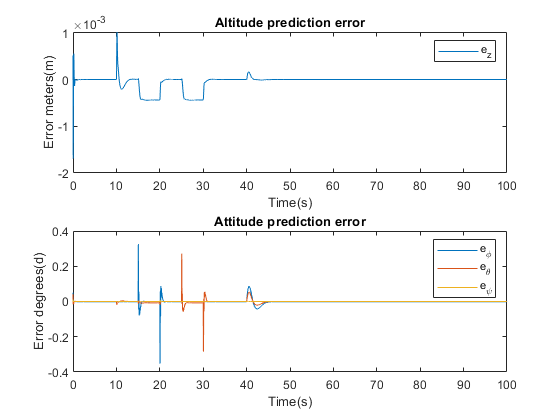
\includegraphics[width=1\textwidth]{ModKFerror.png}	
						\caption{KF Error}
						\label{fig:modifiedkalmanfiltererror}
					\end{minipage}\hfill
					\begin{minipage}{0.5\textwidth}
						\centering
						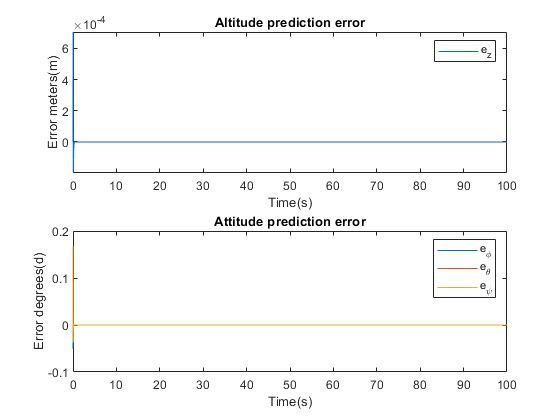
\includegraphics[width=1\textwidth]{ModEKFerror.png}
						\caption{Limited EKF Error}
						\label{fig:limitedxtenderkalmanfiltererror}
					\end{minipage}
				\end{figure}
					
			\subsection{Results}
				
				Figures 4.5 shows the closed-loop system eigenvalues, where after implementation of the designed LQG controller, all eiganvalues are now in within the unit circle, thus stabilising the system. Figures 4.6 to 4.8 show response plots of the system inputs, and both the estimated, with Limited EKF, and measured outputs respectively, as the simulation is run over an interval of 100 seconds. The system is subjected to reference step inputs where the results are displayed in Table 4.1:
				\\ \\
				
				\begin{table}[h!]
					\centering
					\begin{tabular}{ |p{1.5cm}|p{3cm}|p{2cm}|p{2cm}|p{2cm}|p{2cm}|  }
						\hline
						\multicolumn{6}{|c|}{Step Responses} \\
						\hline
						Output   &  Reference  & Overshoot (\%) & Settling Time (s) & Rise Time (s) & Steady State Error \\
						\hline
						Z        &  1 meter         & < 5 &  3   & < 2   & 0\\
						$\phi$   &  30 degrees      & < 5 & < 1  & < 0.5 & 0\\
						$\theta$ &  30 degrees      & < 5 & < 1  & < 0.5 & 0\\
						$\psi$   & 	90 degrees      & 0   & < 5  & < 3   & 0\\
						\hline
					\end{tabular}
					\caption{Table of LQG Step Response values}
					\label{table:lqgstepresponses}
				\end{table}
			
				\begin{figure}[h!]
					\centering
					\begin{minipage}{0.9\textwidth}
						\centering
						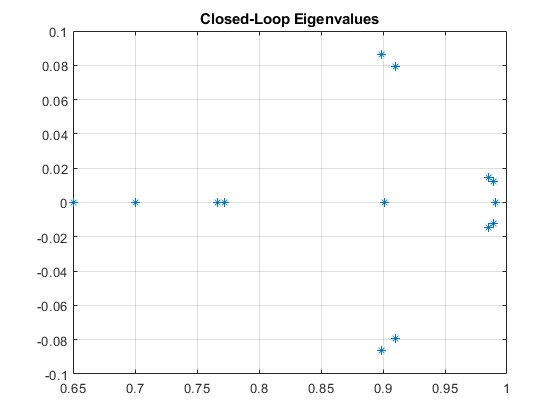
\includegraphics[width=1\linewidth]{DiscreteSystemPoles2.png}
						\caption{Closed-Loop Eigenvalues}
						\label{fig:closedloopeigenvalues}
					\end{minipage}\hfill
					\begin{minipage}{0.9\textwidth}
						\centering
						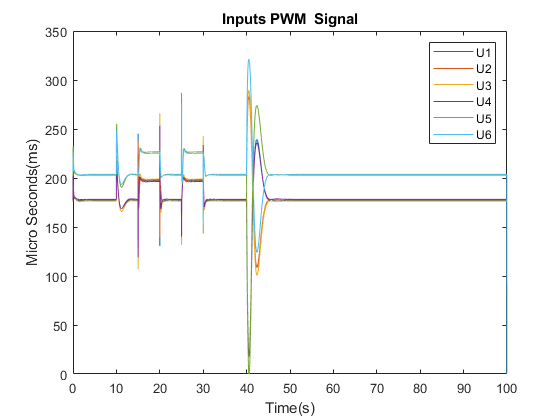
\includegraphics[width=1\textwidth]{LQGEKFInputs.png}	
						\caption{System Input PWM Signal}
						\label{fig:systeminputs}
					\end{minipage}\hfill
				\end{figure}
				
				\begin{figure}[h!]
					\centering
					\begin{minipage}{0.9\textwidth}
						\centering
						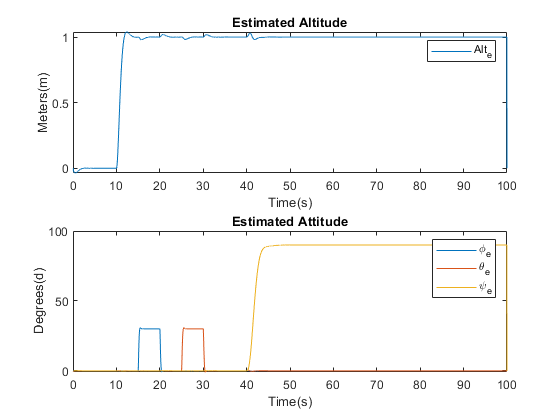
\includegraphics[width=1\textwidth]{ModEKFestOutputs.png}
						\caption{System Estimated Outputs}
						\label{fig:systemestimatedouputs}
					\end{minipage}\hfill
					\begin{minipage}{0.9\textwidth}
						\centering
						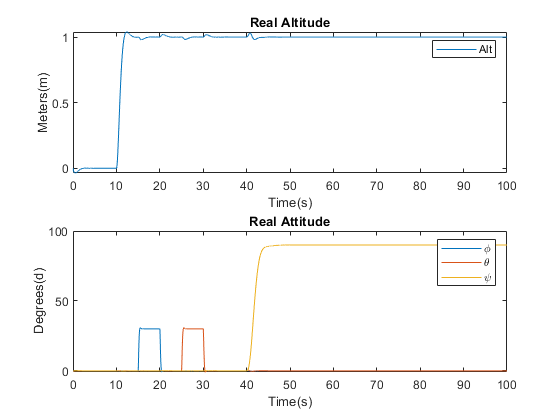
\includegraphics[width=1\textwidth]{ModEKFrealOutputs.png}
						\caption{System Measured Outputs}
						\label{fig:systemmeasuredouputs}
					\end{minipage}
				\end{figure}
			
		\newpage
		
		\section{LQ-MPC}
			
			\subsection{Limitations of LQG control}
				
				\begin{figure}[h!]
					\centering
					\begin{minipage}{0.5\textwidth}
						\centering
						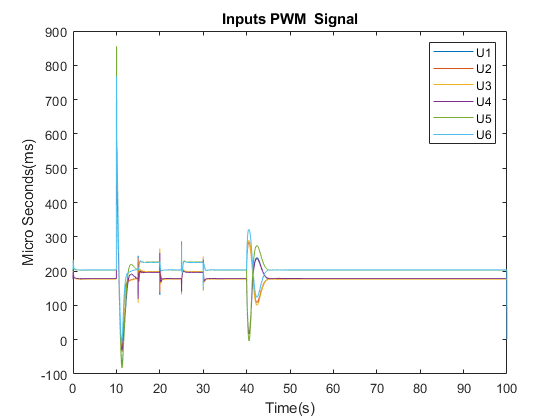
\includegraphics[width=1\textwidth]{LQGInputConstraintViolation.png}
						\caption{Input Constraint Violation}
						\label{fig:inputconstraintviolation}
					\end{minipage}\hfill
					\begin{minipage}{0.5\textwidth}
						\centering
						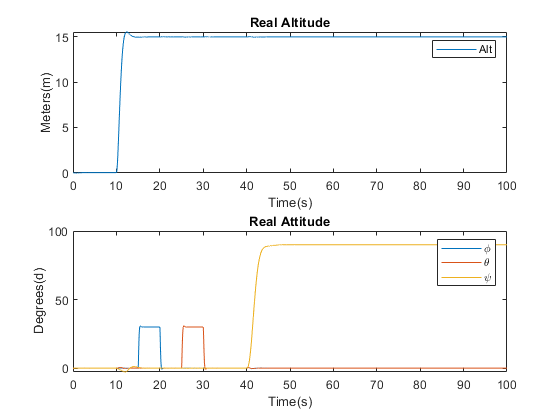
\includegraphics[width=1\textwidth]{LQGOutputConstraintViolation.png}
						\caption{Output Constraint Violation}
						\label{fig:outputconstraintviolation}
					\end{minipage}
				\end{figure}
				
				The LQG is a powerful control mechanism, however, there is one major drowback the using LQG control and that is the inability to taking into account both physical and performance constraint placed on the system states and inputs. This is shown in Figures 4. and 4. where the controller demands and inputs in excess of 800 $\mu_s$ and below 0 $\mu_s$ when a  step change of 15 meters in z is demanded of the system, where 0 to 800 $\mu_s$ is the physical systems input operating range. This could potentially be hazardous if the application where safety critical and the controller were to violate a constraint.
				\\
				Like LQG, MPC techniques are also part of the of optimal control family, however, with MPC implementations, the possibility exists where control signals can be determined such that they implicitly taking into account and produce control action so as to meet system constraints. 
				
			\subsection{General Model Predictive Control (GPC)}
			
				MPC does not refer to any one algorithm or method but instead a methodological philosophy with which to approach control problems, containing certain key concepts and ideas implemented in various ways \cite{26}. There are 3 main components in a GPC algorithm:
				\begin{itemize}
					\item 
						Prediction
					\item
						Optimisation
					\item
						The Receding Horizon Principle
				\end{itemize}
				\space
				The prediction stage of a GPC algorithm uses the model to predict the future system states of the system, if provided with some sequence of control actions. This is dervived by recursively implementing the systems model unto itself to produce a higher order prediction model over a specified horizon length \cite{25},\cite{26},\cite{27}. Given a system of the equation 4.10 form, a state prediction model for a horizon of length N, and evaluated at a time instance k, can be defined as:
				\begin{equation}
					\bar{X}(k) = F X(k) + G \bar{\mu}(k)
				\end{equation}
				where:
				\begin{equation}
					\bar{X}(k) = 
					\begin{bmatrix}
						X(k+1|k)\\
						X(k+2|k)\\
						\vdots\\
						X(k+N|k)
					\end{bmatrix}
					,
					\bar{\mu}(k) = 
					\begin{bmatrix}
						\mu(k|k)\\
						\mu(k+1|k)\\
						\vdots\\
						\mu(k+N-1|k)
					\end{bmatrix}
					,
					F =
					\begin{bmatrix}
						A_{dt}\\
						A_{dt}^{2}\\
						\vdots\\
						A_{dt}^{N}
					\end{bmatrix}
					,
					G =
					\begin{bmatrix}
						B_{dt} & 0 & \dots & 0\\
						A_{dt}B_{dt}& B_{dt}& \dots & 0\\
						\vdots& \vdots & \ddots & \vdots\\ 
						A_{dt}^{N-1}B_{dt}& A_{dt}^{N-2}B_{dt} & \dots & B_{dt}
					\end{bmatrix}
				\end{equation}
				\space
				The Optimisation stage seeks to formulate and solve an optimisation problem \(P_N(X(0))\), to obtain the minimising control sequence over the whole horizon $\bar{\mu}$, evaluated at each time step k, where:
				\(P_N(X(0)) = \)				
				\begin{equation}
					min_\mu  V_N(X(0),\bar{\mu}) = \sum_{i = 0}^{i = N-1} X^{T}(k+i|k) Q X(k+i|k) + \mu^{T}(k+i|k) R \mu(k+i|k)
				\end{equation}
				\(s.t\)
				\[
					X(k|k) = X(k)
				\]
				\[
					X(k+1+i|k) = A_{dt}X(k+i|k) + B_{dt} \mu(k+i|k) , i=1,2,3\dots,N-1
				\]
				Where $Q^{n \times n}$, and $R^{m \times m}$, are 2-norm weighing matrices on the states and inputs respectively. If equation 4.25, is substituted into 4.27, this puts 4.27 into the standard form of a quadratic programming problems where:
				\begin{equation}
					V_N(X(0),\bar{\mu}) = min_\mu \frac{1}{2} \bar{\mu}^{T}(k) H \bar{\mu}(k) + C_q^{T}\bar{\mu}(k) + \alpha
				\end{equation}
				and:
					\[H = 2(G + \tilde{Q}G + \tilde{R})\]
					\[C_q = L X(k) , L = 2 G^{T} \tilde{Q} F\]
				\begin{equation}
					\alpha = X(0)^{T} M X(0), M = F^{T} \tilde{Q} F + Q
				\end{equation}
				With \( \tilde{Q} \) and \(\tilde{R}\) being \(N-1 \times N-1\) dimensional matrix diagonal matrices, with the Q and R matrices as diagonal terms respectively.
				\\
				Solving this Quadratic Program produces a 1 by $mxN$ optimal control sequence of form:
				\begin{equation}
					\bar{\mu }= -H^{-1} L X(k)
				\end{equation}
				where the optimal control gain, $K_N$, consists of the first $m \times n$ terms in the $-H^{-1} L$ due to the implementation of the receding horizon principle. 
				\\
				This is the reason MPC implementations are also known as receding horizon control (RHC) as they only perform the first set of control actions in the sequence $\bar{\mu}$, before recalculating and performing this action at every time interval, k, the target is reached. This continual updating provides feedback into the system \cite{25},\cite{26},\cite{27}. 
				
			\subsection{LQ-MPC: Extending The LQR}
				
				The control law derived,$K_N$ in the previous subsection as opposed to the LQR control law K, derived in the previous section, is not necessarily stabilising even under nominal conditions. This is due to the complex interaction between N,Q,R. \cite{25},\cite{26}. In order to mitigate this, the conditions at the terminal state, k+N, must be made to behave in a similar way as the infinite horizon LQR.
				\\
				The is accomplish through the addition of an optimal terminal cost, P, to the cost function \(P_N(X(0))\). This then becomes: 
				\begin{equation}
					min_\mu  V_N(X(0),\bar{\mu}) = \sum_{i = 0}^{i = N-1} [ X^{T}(k+i|k) Q X(k+i|k) + \mu^{T}(k+i|k) R \mu(k+i|k) ] + X^{T}(k+N|k) P X (k+N|k)
				\end{equation}
				\(s.t\)
				\[
					X(k|k) = X(k)
				\]
				\[
					X(k+1+i|k) = A_{dt}X(k+i|k) + B_{dt} \mu(k+i|k) , i=1,2,3\dots,N-1
				\]
				This also changes\( \tilde{Q} \) to include P as another diagonal term, making it \(N \times N\) dimensional.
				\\ \\
				The value of P is derived through satisfying the application of the Lyapunov equation:
				\begin{equation}
					(A_{dt} + B K)^{T} P (A_{dt} + B K) - P = T
				\end{equation}
				Where T is the infinite horizon cost and K is the LQR gain. Therefore, with the addition of P, if K is stabilising then, $K_N$ is guaranteed asymptotically stabilising in the unconstrained case \cite{26}. provided the system is 
				\begin{itemize}
					\item 
						Stabilisable
					\item
						Observable
					\item
						Q is at least P.S.D and R is P.D
				\end{itemize}
				\space
				This form of MPC is also know as dual mode-MPC as the controller is in effect switching between one set of control laws when far from the steady state, k < N, and another when near it, K $\geq$ N. \cite{25},\cite{26},\cite{27}.
				
			\subsection{Closed-Loop Predictions}
				
				The Closed-loop paradigm embeds the optimal stabilising controller gains, K, into the prediction model of the system, pre-stabilising and in doing to defines a new control variable, c, a perturbations about the embedded most desired performance  where:
				\begin{equation}
					\mu(k+i-1) = -K X(k+i-1) + c(k+i-1), i = 1,2,\dots,N
				\end{equation}
				This paradigm is known as Optimal-MPC (OMPC) and  produces a control implementation structure of the form shown in Figure 4.11, \cite{26}.
				
				\begin{figure}[h!]
					\centering
					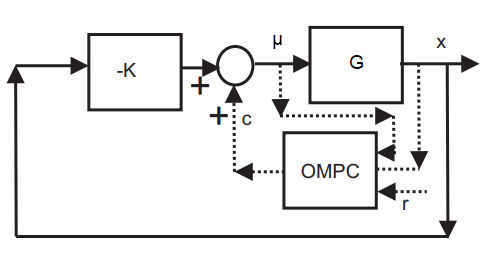
\includegraphics[width=0.8\linewidth]{OMPC.png}
					\caption{OMPC Implementation Structure}
					\label{fig:ompcimplementationstructure}
				\end{figure}
			
				When equation 4.33 is substituted into equations 4.25 and 4.32, this produces the quadratic programming problem:
				\begin{equation}
					min_c V_N(X(0)) = c^{T}(k) S_c c(k) + 2 c^{T}(k) S_{cx}X(k)
				\end{equation}
				Which when solved produces:
				\begin{equation}
					\bar{c}(k) = - S_c^{-1}S_{cx}X(k)
				\end{equation}
				This provide the closed-loop paradigm control law in the unconstrained case:
				\begin{equation}
					\mu(k) = - [K + S_c^{-1}S_{cx}]X(k)
				\end{equation}
				The implementation of the Closed-loop paradigm is especially important when dealing with unstable systems,such as multirotors, as large prediction horizons N, the prediction matrices, F and G, may become numerically ill-conditioned leading to control implementation issue especially in embedded systems with limited computational power. However, the incorporation of the stabilising feedback K, into the prediction matrices changes their conditioning\cite{26},\cite{27}.
				
			\subsection{Reference Tracking}
				
				\begin{figure}[h!]
					\centering
					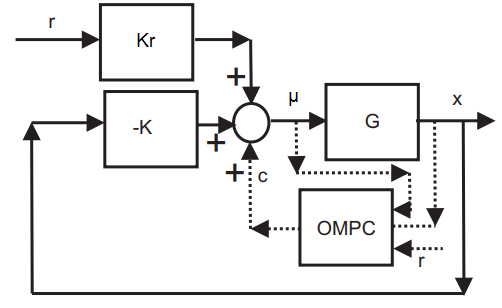
\includegraphics[width=0.8\linewidth]{OMPC2.png}
					\caption{OMPC Implementation Structure}
					\label{fig:ompcimplementationstructure}
				\end{figure}
				Reference tracking is achieved through the implementation of deviation variable. These are the state and input values at the desired target state where the equilibrium inputs $\mu_e$, and the reference signal r, make up these variable. where we define an $1 \times n$ vector Xr, which contains the output references and state equilibrium point:
				\begin{equation}
					\begin{bmatrix}
						r_1(k)&0&r_2(k)&0&r_3(k)&0&r_4(k)&0&\omega_e1&\omega_e2&\omega_e3&\omega_e4&\omega_e5&\omega_e6
					\end{bmatrix}
				\end{equation}
				
				A control law of form:
				\begin{equation}
					\mu(k) = - [K + S_c^{-1}S_{cx}]( X(k)- Xr) + \mu_e
				\end{equation}
				In the unconstrained case, $S_{cx}$ = 0, therefore the unconstrained Closed-Loop paradigm LQ-MPC, results in state feedback \cite{26}.
				
			\subsection{Results}
				Figures 4.13 to 4.16 show response plots of the system inputs, system perturbations, and both the estimated, with Limited EKF, and measured outputs respectively, as the simulation is run over an interval of 50 seconds. The system is subjected to reference step inputs where the results are displayed in Table 4.2:
				\\
				\begin{table}[h!]
					\centering
					\begin{tabular}{ |p{1.5cm}|p{3cm}|p{2cm}|p{2cm}|p{2cm}|p{2cm}|  }
						\hline
						\multicolumn{6}{|c|}{Step Responses} \\
						\hline
						Output   &  Reference  & Overshoot (\%) & Settling Time (s) & Rise Time (s) & Steady State Error \\
						\hline
						Z        &  1 meter         & < 5 &  3   & < 2   & 0\\
						$\phi$   &  30 degrees      & < 5 & < 1  & < 0.5 & 0\\
						$\theta$ &  30 degrees      & < 5 & < 1  & < 0.5 & 0\\
						$\psi$   & 	45 degrees      & 0   & < 5  & < 3   & 0\\
						\hline
					\end{tabular}
					\caption{Table of LQ-MPC Step Response values}
					\label{table:lqmpcstepresponses}
				\end{table}
				
				\begin{figure}[h!]
					\centering
					\begin{minipage}{0.5\textwidth}
						\centering
						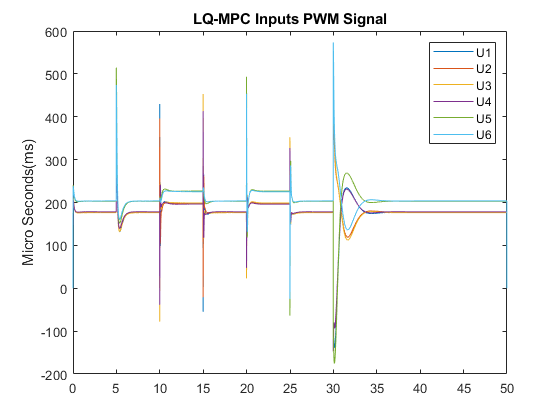
\includegraphics[width=1\textwidth]{LQMPCInputs.png}
						\caption{LQ-MPC Unconstrained Inputs}
						\label{fig:lqmpcunconstrainedinputs}
					\end{minipage}\hfill
					\begin{minipage}{0.5\textwidth}
						\centering
						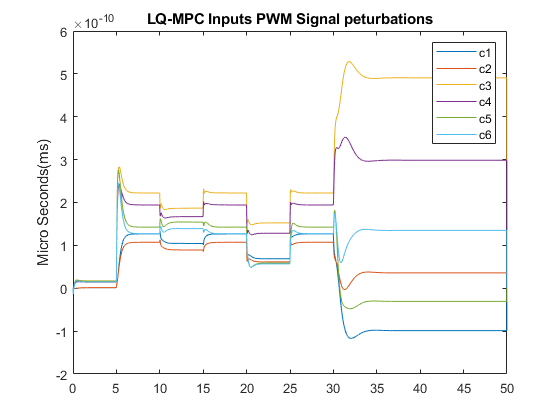
\includegraphics[width=1\textwidth]{LQMPCPerturbations.png}
						\caption{LQ-MPC Unconstrained Perturbations}
						\label{fig:lqmpcunconstrainedperturbations}
					\end{minipage}
				\end{figure}
			
				\begin{figure}[h!]
					\centering
					\begin{minipage}{0.5\textwidth}
						\centering
						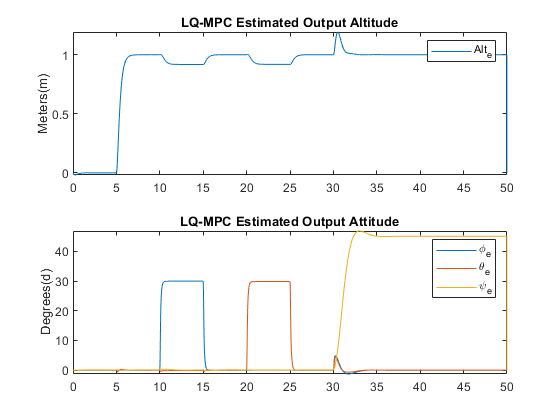
\includegraphics[width=1\textwidth]{LQMPCestOutputs.png}
						\caption{LQ-MPC Estimated Outputs}
						\label{fig:lqmpcestimatedoutputs}
					\end{minipage}\hfill
					\begin{minipage}{0.5\textwidth}
						\centering
						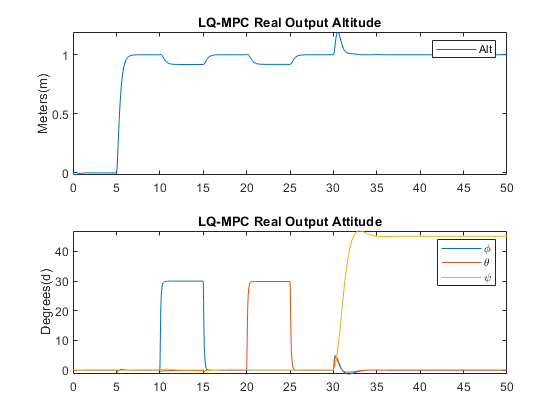
\includegraphics[width=1\textwidth]{LQMPCrealOutputs.png}
						\caption{LQ-MPC Model Outputs}
						\label{fig:lqmpcrealoutputs}
					\end{minipage}
				\end{figure}
			
			\newpage
			
		\section{Summary}
			
			This Chapter:
			\begin{itemize}
				\item 
					Converted the Linearised model into a for suitable for control analysis and design
				\item 
					Analysed key system properties such as its stability in open loop, reachability and observability 
				\item
					Discussed and derived full-state feedback control and the application of the LQR producing optimal feedback
				\item
					Discussed the necessity for state estimation and proposed a modified Kalman filter for state estimation thus producing an LQG controller whose performance was tested and results presented
				\item
					Discussed limitations of the LQG and presented and derived an LQ-MPC controller as a solution, whose performance was tested and results presented.
			\end{itemize}
		
	\newpage
		
	\chapter{Embedded Control Systems Implementation}
		
		\section{Introduction}
			
			Advanced control systems need to be implemented using digital computers. In an application such as with UAVs, this computation needs to occurs on a devices as physically small as possible, due to design consideration such as minimising total vehicle mass. One such class of applicably small computers are SBCs. These are usually fully capable computers in their own right running light weight operating systems, such as some version watered down Linux distributions. Many typically have smaller physical dimension comparable to that of debit cards. Such devices have become possible and previlent due to the advent of smartphone technology driving the trend towards cost effective minimisation of processing units. 
			\\
		 	This chapter will go through the considerations and processes involved in implementing control systems and propose an implementation, via a systems engineering framework, of a flight control system. These considerations are:
			
			\begin{enumerate}
				\item
					Hardware
				\item
					Sensors
				\item
					Software Libraries
				\item 
					UML Implementation
			\end{enumerate}  
			
		\section{Hardware}
			
			\begin{figure}[h!]
				\centering
				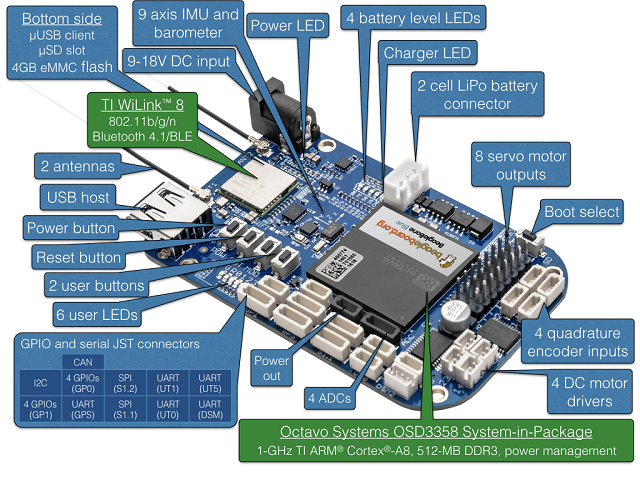
\includegraphics[width=1\linewidth]{beagle-bone-blue-annotated.png}
				\caption{BeagleBone Blue SBC}
				\label{fig:beaglebonebluesbc}
			\end{figure}
		
			The SBC under consideration for the project is the Beagle Bone Blue (BBB) from the BeagleBoard group, shown in Figure 5.1, which, in addition to the computation provided by all SBCs, has been developed with many additional features that make is suitable for implementation in robotics.
			\\
			The BBB possesses a 1 Gigahertz ARM Cotrex-A8 mirco-processor unit, supported by 512 Megabytes of DDR3 random access memory (RAM). This SCB is also capable of wireless communication through various Bluetooth and Wi-Fi standards. However for the purposes of this investigation all communication to the SBC will occurs via a radio transmitter to a waiting receiver onboard the UAV. This transmitter will effectively be sending the reference commands, r, to the controller which will be read in as Pulse Position Modulated (PPM) values by the SBC. 
			\\
			The BBB comes equipped with multiple, peripheral communication interfaces such as:
			\\
			\begin{itemize}
				\item
					Inter-Integrated Circuit ($I^{2}C$)
				\item
					Serial Periheral interface (SPI)
				\item
					 Genral Purpose Input-Outputs (GPIOs) at 3.3v Logic Level ($V_{op}$)
				\item
					Universal Asynchronous receiver-Transmitter (UART) 
			\end{itemize}  
			
			The BBB also comes equipped with multiple sensor, the addition of which, are the most pertinent hardware inclusions with regards to this investigation. These are:
			\\
			\begin{itemize}
				\item
					A Magnetic, Angular rate, Gravity Sensor (MARG)
				\item
					A Barometric Pressure Sensor (Barometer/Baro)
			\end{itemize}  
			
			\subsection{MARG and Barometer}
			
				A MARG sensor consists of a 3-axis gyroscope, which measures angular rate, a 3-axis accelerometer which measure linear acceleration, and a 3-axis magnetometer which measures the strength of the earth's magnetic field. 
				\\
				Barometers are sensors which measure atmospheric pressure. their use on UAVs is key as pressure on the surface of the earth is a function of the altitude, therefore the pressure readings from a barometer can be used to estimate the altitude above sea-level of a body \cite{20},\cite{29}.
				\\
				When combined, the sensors can be used to estimate the angular position and altitude of the body they are attached to. In the form factor able to be implemented on an SBC, MARGs come as mirco elctro-mechanical systems (MEMS) sensors which take the form of integrated circuits. MEMS devices contain moving masses and are able to convert the movement of these masses into readable data \cite{20},\cite{29}. The MARG implemented here is the MPU-9650 from innovosense and the Barometer is the BPM-280 from BOSH.
				\\
				In order to be used these devices they must be calibrated to remove bias and offset errors due to the effect of external disturbances, especially on MEMS devices \cite{29}. 
				
			\subsection{Actuator interfaces}
			
				Broken out of the board through its GPIO pin header, are 8 serve motor controller port, as show in figure 5.1, which are able to generate PWM signals and interface with ECSs. These pins will be used to interface with the propulsion units.
				
		\section{Software and UML}
		
			\subsection{The Robot Control Library (RCL)}
			
				\begin{figure}[h!]
					\centering
					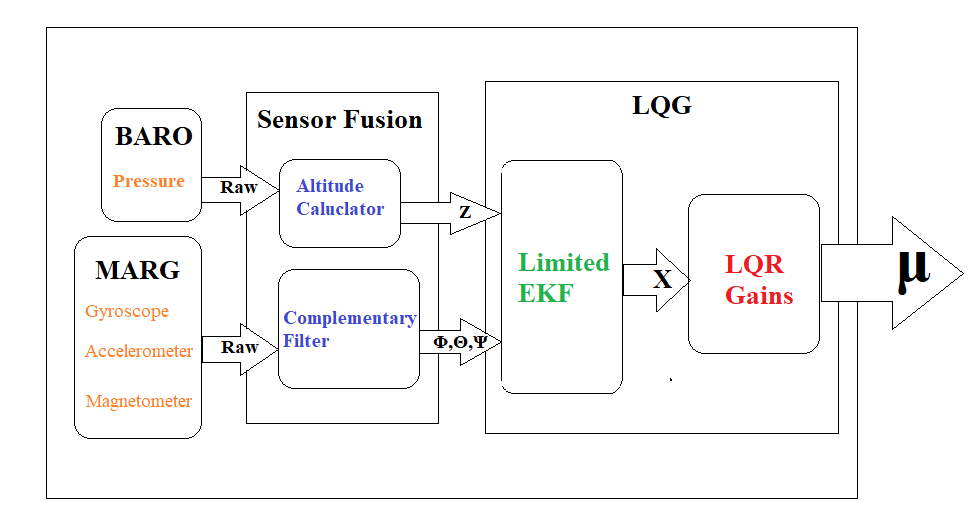
\includegraphics[width=1\linewidth]{ImplementationStructure.png}
					\caption{Embedded Component Structure}
					\label{fig:embeddedcomponentstructure}
				\end{figure}
			
				The BBB is an embedded Linux SBC running a customised Linux distribution which comes included with the RCL. The RCL is the primary software package for interfacing with and developing robotics software for the BBB and other BeagleBoard group SBCs. This package contains libraries written in the C programming language that provide an application programming interface (API) for accessing the sensors and communication interfaces for the Robot Control projects \cite{31} The package also conveniently comes with examples and testing programs . 
				\\ \\
				This package includes an extensive mathematics library for performing discrete-time feedback control such as including functions for:
				
				\begin{itemize}
					\item
						KF and EKF implementation.
					\item
						Digital Signal Processing and Filtering.
					\item
						Sensor Fusion Algorithms.
				\end{itemize}  
		
				Besides these functions, the package also comes with various timing, multithreading and program flow functions, all of which is aimed at developing robotics software on embedded platforms.
				\\
				Using the functions provided by the RCL, a basic implementation structure can be developed, as show in Figure 5.2, where:
				\\
				\begin{enumerate}
					\item 
						Raw sensor values are read in by the SBC
					\item 
						These value are passed through a sensor fusion stage which calculates $Z$ from raw pressure values and combines then converts the MARG value into $\phi,\theta\psi$ through a sensor fusion algorithm, the complementary filter \cite{20}, to make up the measured outputs Y.
					\item 
						Y is then sent to the Limited EKF developed in Chapter 4, the Limited EKF then returns the full state, X
					\item 
						X is then augmented with the integral term and multiplied with the LQR gains developed in chapter 4 to produce the input vector $\mu$.
				\end{enumerate}
			
			\subsection{Universal Modelling Language (UML)}
			
				UML is an Industry standard set of tools which consists of a set of different diagram types, which is used to model software system \cite{30}.
				\\
				The specific UML diagram implemented here is the UML class diagram. This diagram type is used to represent sections of software while showing the relationship between the different section. Class diagrams are typically utilised to represent system developed in an object-oriented manner with functionality separated into different classes, such as is possible with software developed in the C++ or the Java languages amongst many others \cite{30}. 
				\\
				However, class diagrams can be adapted to represent systems developed in a non-object oriented programming environments, such as the C language, if the functionality is sufficiently encapsulated and atomised. This is presented in Figure 5.3
				\\
				The Presented UML diagram show key functionality grouped into blocks, as shown in Figure 5.2. Each block contaits Function extracted from the RCL Library which perform the blocks desired function \cite{31}.
				\\
				\begin{itemize}
					
					\item 
						The Sensor.h block shows the functions for reading in data from the MARG and Barometer
					\item 
						The SensorFusion.h block show functions from implementing a complementary and a built-in library script or calculating the altitude from pressure.
					\item
						The LimitedEKF.h shows functions for implementing an extended Kalman filter.
					\item
						The Receive.h block show functions which read in and parse through data sent by a radio transmitter using PPM
					\item
						The MotorControl.h block show functions for calibrating the propulsion unit ESCs and sending commands to them.
				\end{itemize}
			
				These blocks are then aggregated in the main.c block
				\\
				
				\begin{figure}[h!]
					\centering
					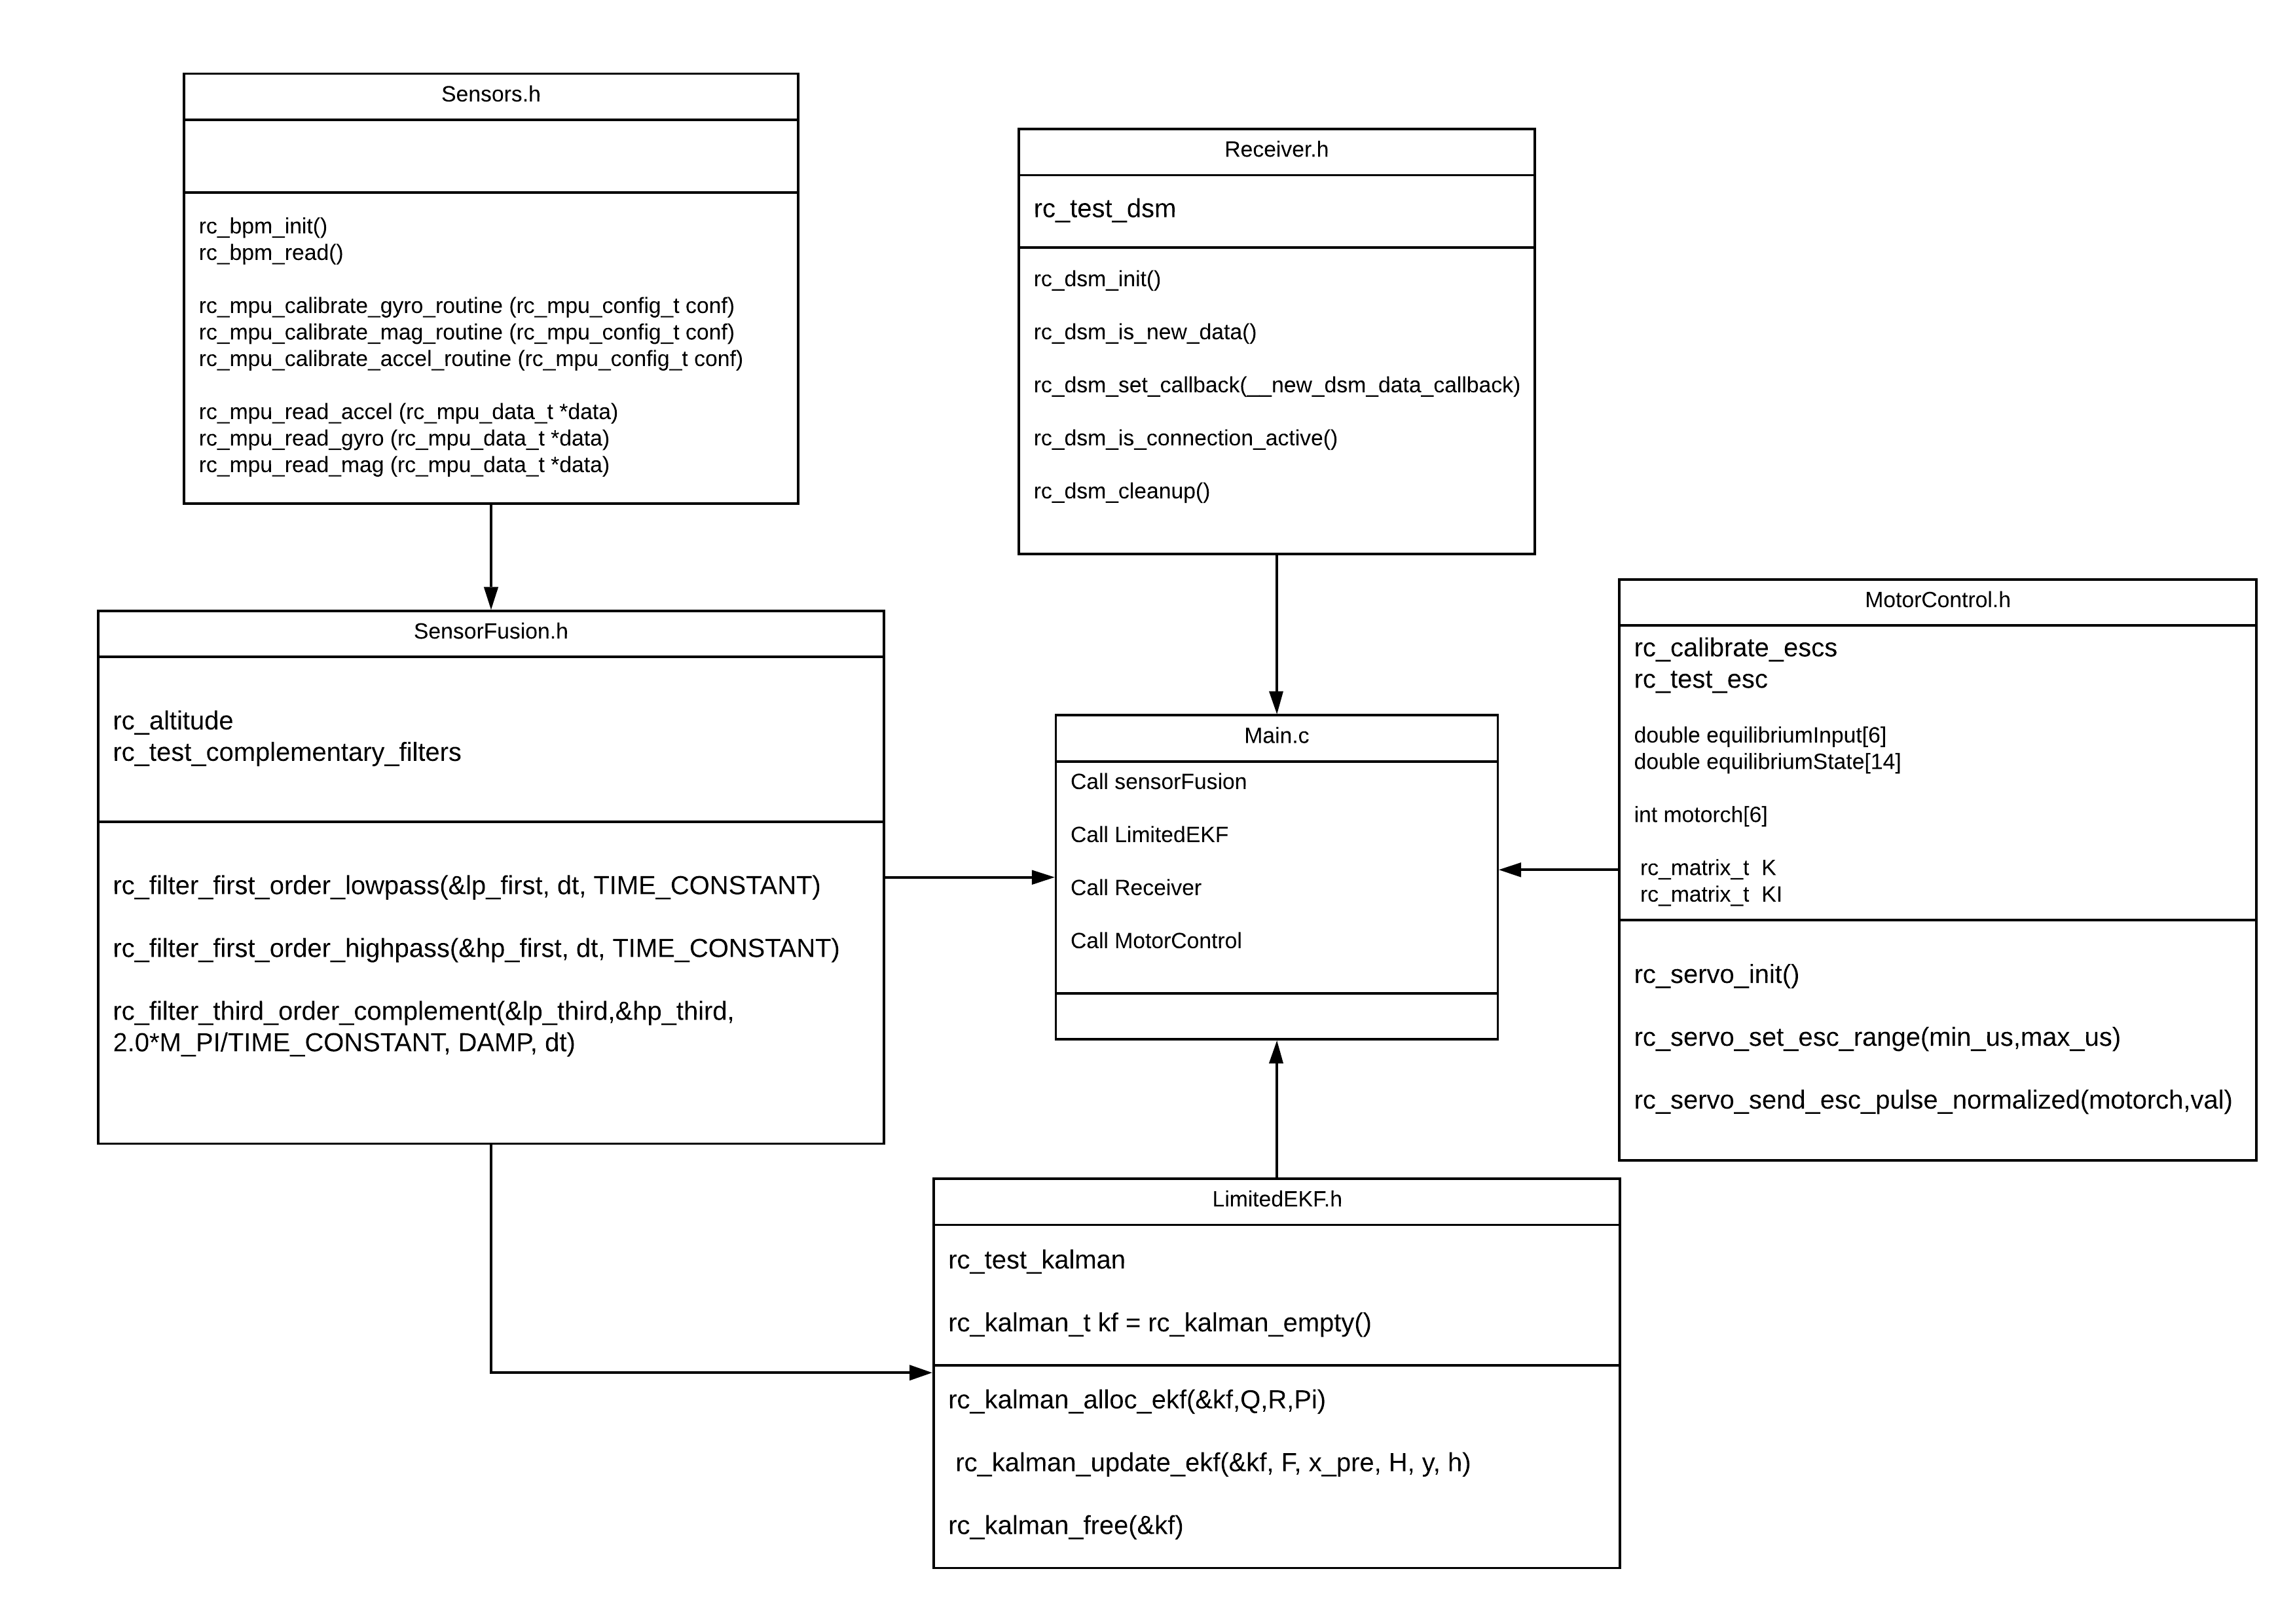
\includegraphics[width=1\linewidth]{LQG-UML-Implementation.png}
					\caption{UML Class diagram of Functions}
					\label{fig:umlfunctiondiagram}
				\end{figure}
				  
				
		\section{Summary}	
			
			This Chapter:
			\begin{itemize}
				\item 
					Discussed the utilisation of Single Board Computers 
				\item 
					Discussed key software and hardware elements available on the Beagle Bone Blue Single Board Computer  
				\item
					Proposed and described an embedded flight control system implementation using the Unified Modelling Language's class diagram framework.
			\end{itemize}
		
	\newpage
	
	\begin{table}[h!]
		\centering
		\begin{tabular}{ |p{1.5cm}|p{9.5cm}|p{5cm}|  }
			\hline
			\multicolumn{3}{|c|}{Control and Implementation Parameters} \\
			\hline
			Character& Definition  & Value  \\
			\hline
			T        &  Discrete Sample Time                        & 0.01 s\\
			DAC      &  Digital to Analog converter resolution      & 10 bits\\
			ADC      &  Analog to Digital converter resolution      & 10 bits\\
			$V_{op}$ & 	SBC Operating Voltage                       & 3.3 v\\
			\hline
		\end{tabular}
		\caption{Table of Control and Implementation Parameters}
		\label{table:controlparameters}
	\end{table}

	\newpage
	
	\chapter{Conclusion}
		
		In conclusion, this investigative project was abled to:
		\begin{enumerate}
			\item
				Develop a mathematical model representing the dynamics of the multirotor aircraft.
			\item
				Convert the model into formats which that could be used for, analysis and control systems design using linear analysis and design techniques, and implementation unto digital embedded systems. 
			\item
				Investigate, develop and implement model-based LQG and LQ-MPC feedback control schemes in simulation.
			\item
				Develop a proposal for implementing LQG based flight control software on an embedded microprocessor unit, conveyed using industry the standard UML software systems modelling tool.
		\end{enumerate}
		Potential Future developments could include:
		\begin{enumerate}
			\item
				Implement the proposed flight control software onto an embedded microprocessor then developing and implementing the developed LQ-MPC control scheme.
			\item
				Re-modelling the system using Quarternions to eliminate to possibility of singularity formation, thus opening up the full range of UAV motion
			\item	
				Investigate and develop non-linear control techniques capable of taking advantage of full motion range provide by a Quarternion based model 
			\item	
				Implementing full control over 3-D euclidean space by incorporating feedback control authority over x and y. \cite{1}
			\end{enumerate}
	
	\newpage
	
	\pagenumbering{roman}
				
	\bibliography{ProjectResearchPapers}
	\bibliographystyle{acm}
	%\bibliographystyle{ieeetr}	
	
	\newpage
	\chapter*{Appendix A: Gantt Chart}
		
		\newpage
		
			\begin{figure}[h!]
				\centering 
				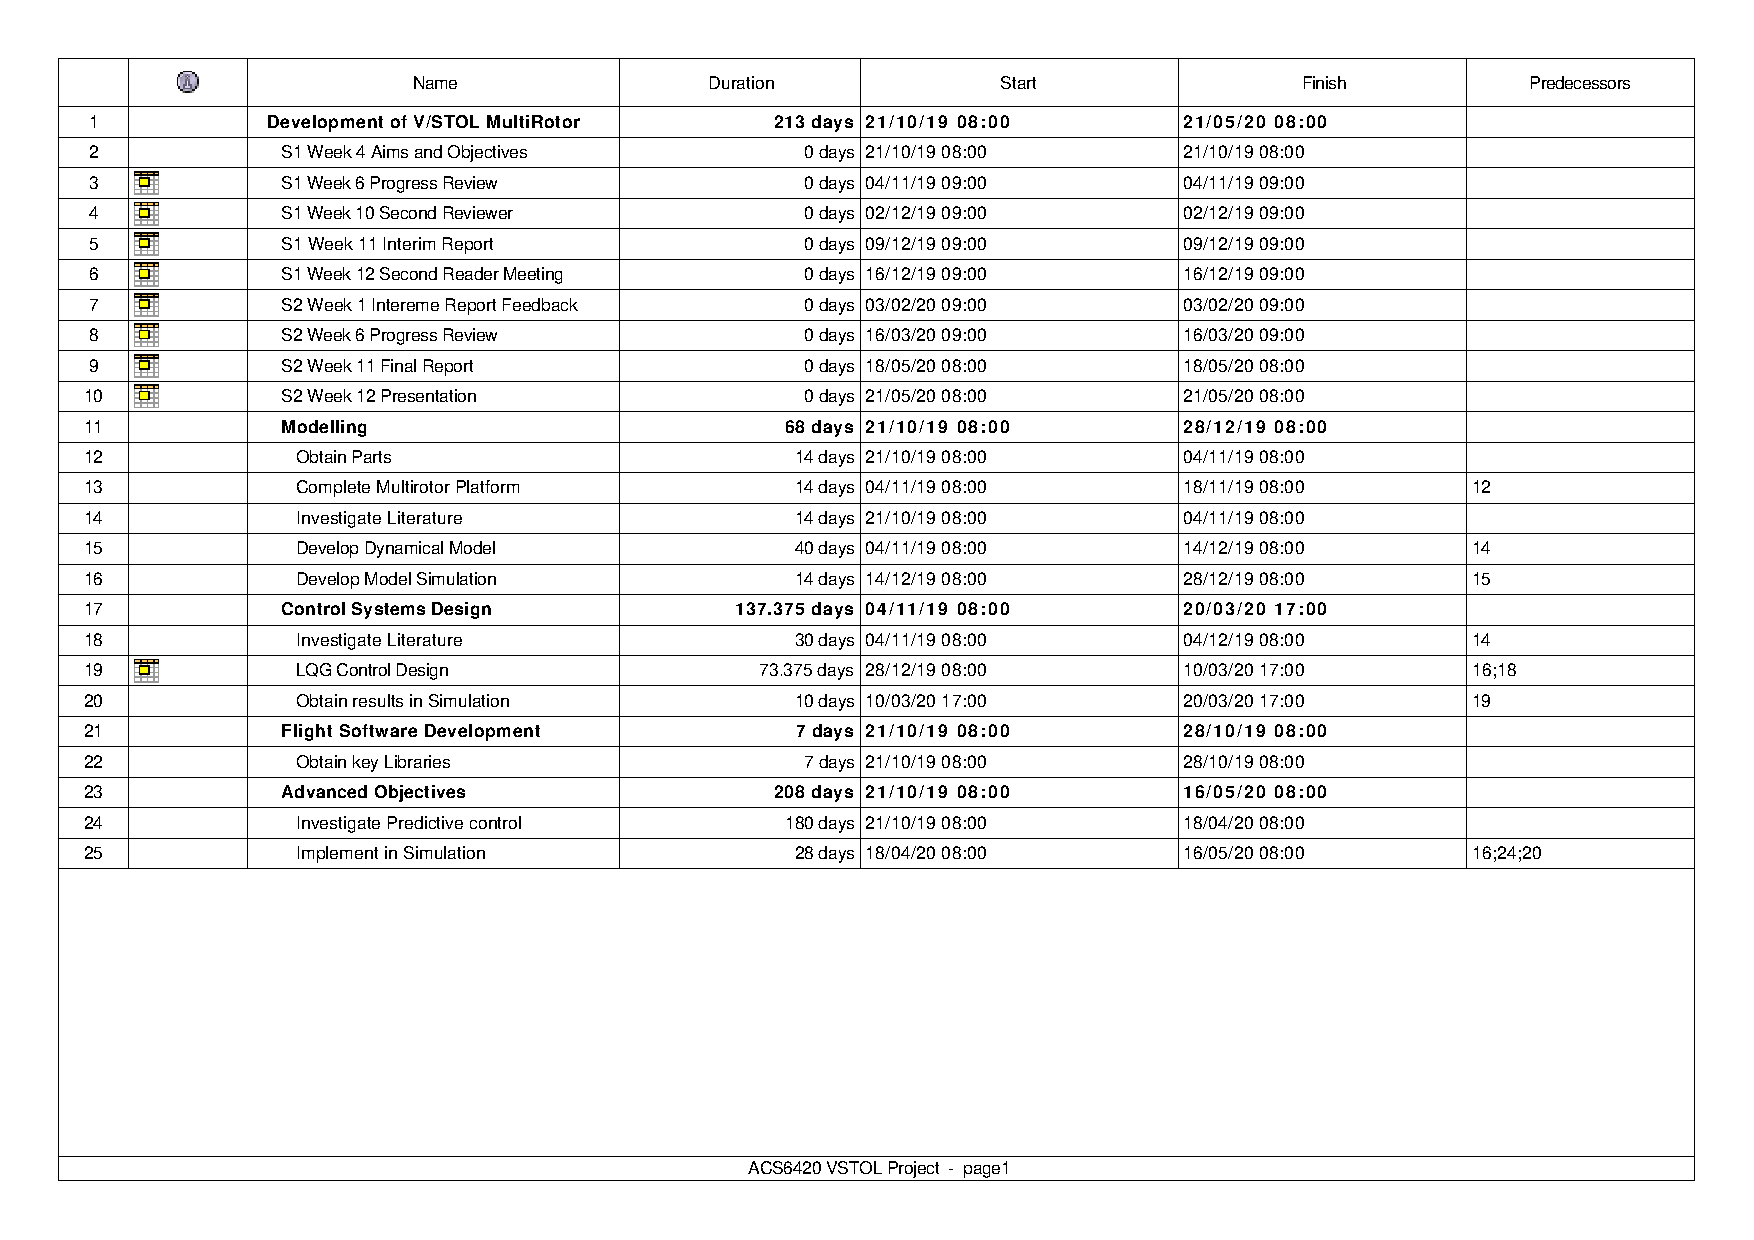
\includepdf[pages=1,pagecommand={},offset=0cm 0cm]{Gantt}
				\caption{Gantt Table of Project Objectives and Dates}
				\label{fig:Gantt Objectives and Dates}
			\end{figure}
			
			\newpage
			
			\begin{figure}[h!]
				\centering 
				\includepdf[pages=2,pagecommand={},offset=0cm 0cm]{Gantt}
				\caption{Gantt Chart Page 1}
				\label{fig:Gantt Chart Page 1}
			\end{figure}
			
			\newpage
			
			\begin{figure}[h!]
				\centering 
				\includepdf[pages=3,pagecommand={},offset=0cm 0cm]{Gantt}
				\caption{Gantt Chart Page 2}
				\label{fig:Gantt Chart Page 2}
			\end{figure}
			
			\newpage
			
			\begin{figure}[h!]
				\centering 
				\includepdf[pages=4,pagecommand={},offset=0cm 0cm]{Gantt}
				\caption{Gantt Chart Page 3}
				\label{fig:Gantt Chart Page 3}
			\end{figure}
		
			\newpage
			
			\begin{figure}[h!]
				\centering 
				\includepdf[pages=5,pagecommand={},offset=0cm 0cm]{Gantt}
				\caption{Gantt Chart Page 4}
				\label{fig:Gantt Chart Page 4}
			\end{figure}
		
	\chapter*{Appendix B: Control Design Parameters}
	
		\setcounter{MaxMatrixCols}{18}
		\begin{equation}
			Q_{LQG} = diag(200,500,1000,10,1000,15,1000,10,0,0,0,0,0,0,1,35,35,0.1)  
		\end{equation}
		
		\begin{equation}
			Q_{LQ-mpc} = diag(500,0,1000,0,1000,0,1000,0,0,0,0,0,0,0)
		\end{equation}
		
		\begin{equation}
			R = diag(10^{-3},10^{-3},10^{-3},10^{-3},10^{-3},10^{-3})
		\end{equation}
		
		\begin{equation}
			\mu_e = (176.1, 178.5, 177.2, 177.6, 202.2, 202.4)
		\end{equation}
		
		\begin{equation}
			\omega_e = \mu_e \times K_u 
		\end{equation}
		
\end{document}